\documentclass[UTF8,12pt]{ctexart}
\usepackage[a4paper, left=2.5cm, right=2.5cm, top=2.5cm, bottom=2.0cm]{geometry} % 调整页面大小
\usepackage{indentfirst} % 每段自动首行缩进
\usepackage{graphicx} % 插入图片
\usepackage{float} % 控制图片位置
\usepackage{amsmath} % 数学公式
\usepackage{listings} % 代码块
\usepackage{xcolor} % 颜色
\usepackage{hyperref} % 超链接
\usepackage{booktabs} % 表格
\usepackage{multirow} % 表格多行
\usepackage{subcaption} % 子图

% 设置图片路径
\graphicspath{{img/}}

\title{基于多源日志的可视化威胁情报分析}
\author{张宏彬,高宇润,王宇,曹家赫}

\begin{document}
\maketitle

\section{问题驱动的方法论框架}
针对本题的可视化需求,我们提出\textbf{"数据-模型-认知"三层分析框架}:
\begin{equation}
\mathcal{F} = \underbrace{\mathcal{D}_{\text{fusion}}}_{\text{数据层}} \circ \underbrace{\mathcal{M}_{\text{threat}}}_{\text{模型层}} \circ \underbrace{\mathcal{V}_{\text{interactive}}}_{\text{认知层}}
\end{equation}

\subsection{数据预处理与特征工程}
在数据层面,我们采用了系统化的数据预处理方法,重点解决数据异构性、时序一致性和特征表达等关键问题。首先,针对文本密集型的邮件日志,我们基于自然语言处理技术构建了完整的文本分析流水线。该流水线首先通过jieba分词系统进行中文分词,随后结合TF-IDF向量化方法提取主题特征。为提高特征的表达能力,我们专门设计了针对企业场景的停用词表,不仅包含常见虚词(如"的"、"了"等),还包含了系统账号(如"kaoqin"、"fuli"等)的过滤规则,从而确保提取的特征具有明确的业务语义。

\begin{figure}[H]
    \centering
    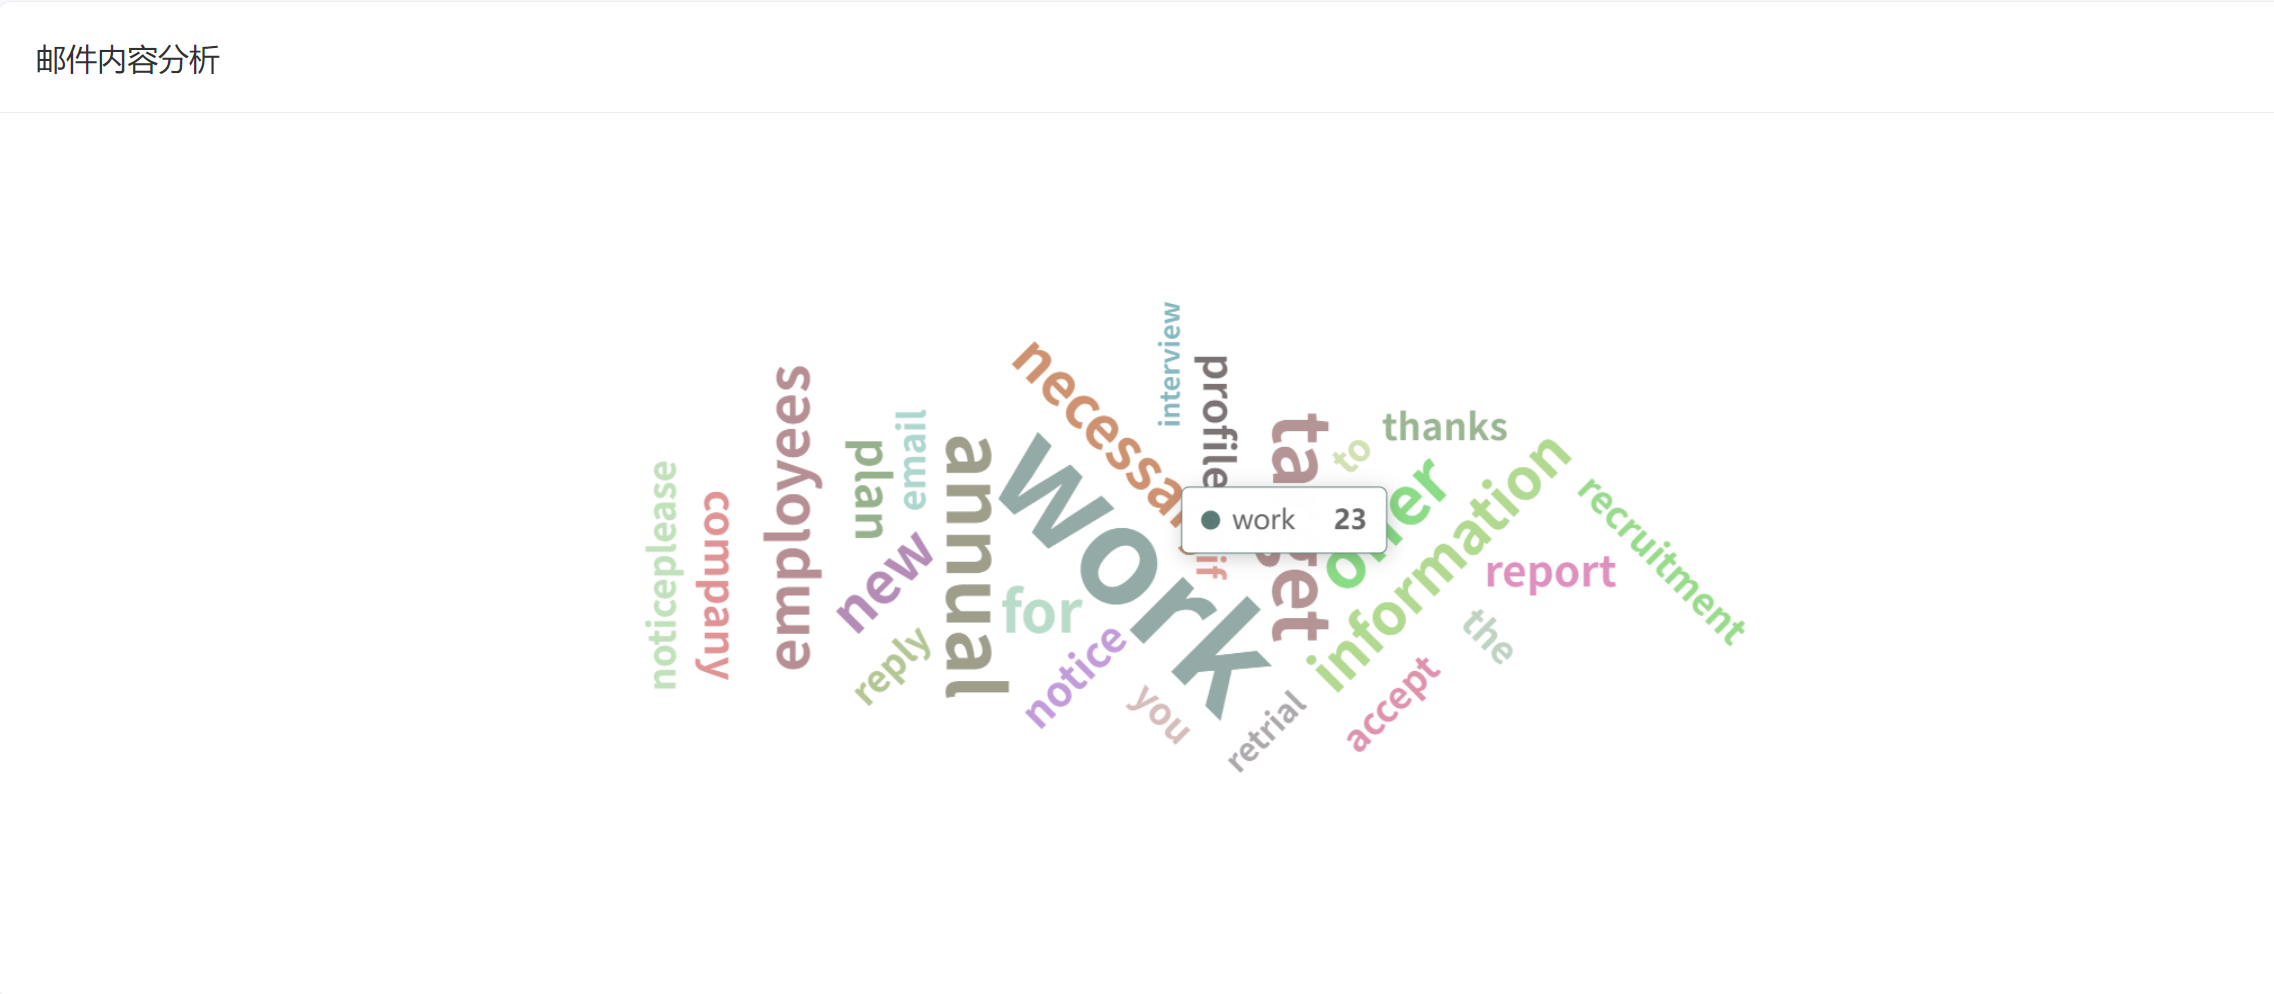
\includegraphics[width=0.8\textwidth]{person_wordcloud.png}
    \caption{员工邮件主题词云图(展示主要业务关键词分布)}
    \label{fig:person_wordcloud}
\end{figure}

在时序数据处理方面,我们重点解决了登录日志中的时间标准化问题。通过设计正则表达式模式库,系统可以识别和统一处理多种日期时间格式(如"2017/11/1 9:21"等),并将所有时间戳规范化到统一的时区和格式。这种标准化不仅便于后续的时序分析,还为多源数据的关联分析奠定了基础。

对于网络行为数据,我们开发了一套分层的网站分类体系。该体系基于域名特征和访问模式,将网站划分为工作相关(如github.com、stackoverflow.com)、技术社区(如csdn.net、juejin.cn)、云存储/文件共享(如dropbox.com、mega.nz)等类别。特别地,我们通过机器学习方法训练了一个域名风险评估模型,该模型能够基于域名的字符分布、注册信息和历史信用记录等特征,对新出现的域名进行风险等级评估。

在网络流量分析方面,我们突破了传统的单维度流量统计方法,提出了多维度的流量特征提取框架。该框架不仅计算基本的流量统计特征(如上下行流量比率),还结合预定义的服务器/数据库IP端口映射表(如"192.168.1.100:3306"对应"Main DB"),构建了服务访问关系图谱。这种方法能够有效捕获异常的数据访问模式,为后续的威胁检测提供更丰富的特征支持。

\subsection{多维度分析模型}
在模型层面,我们构建了一个多层次、多维度的分析框架,以实现对企业内部威胁的全面感知和精准识别。该框架的核心包含三个关键组件:组织结构识别、行为模式建模和异常检测策略。

\begin{figure}[H]
    \centering
    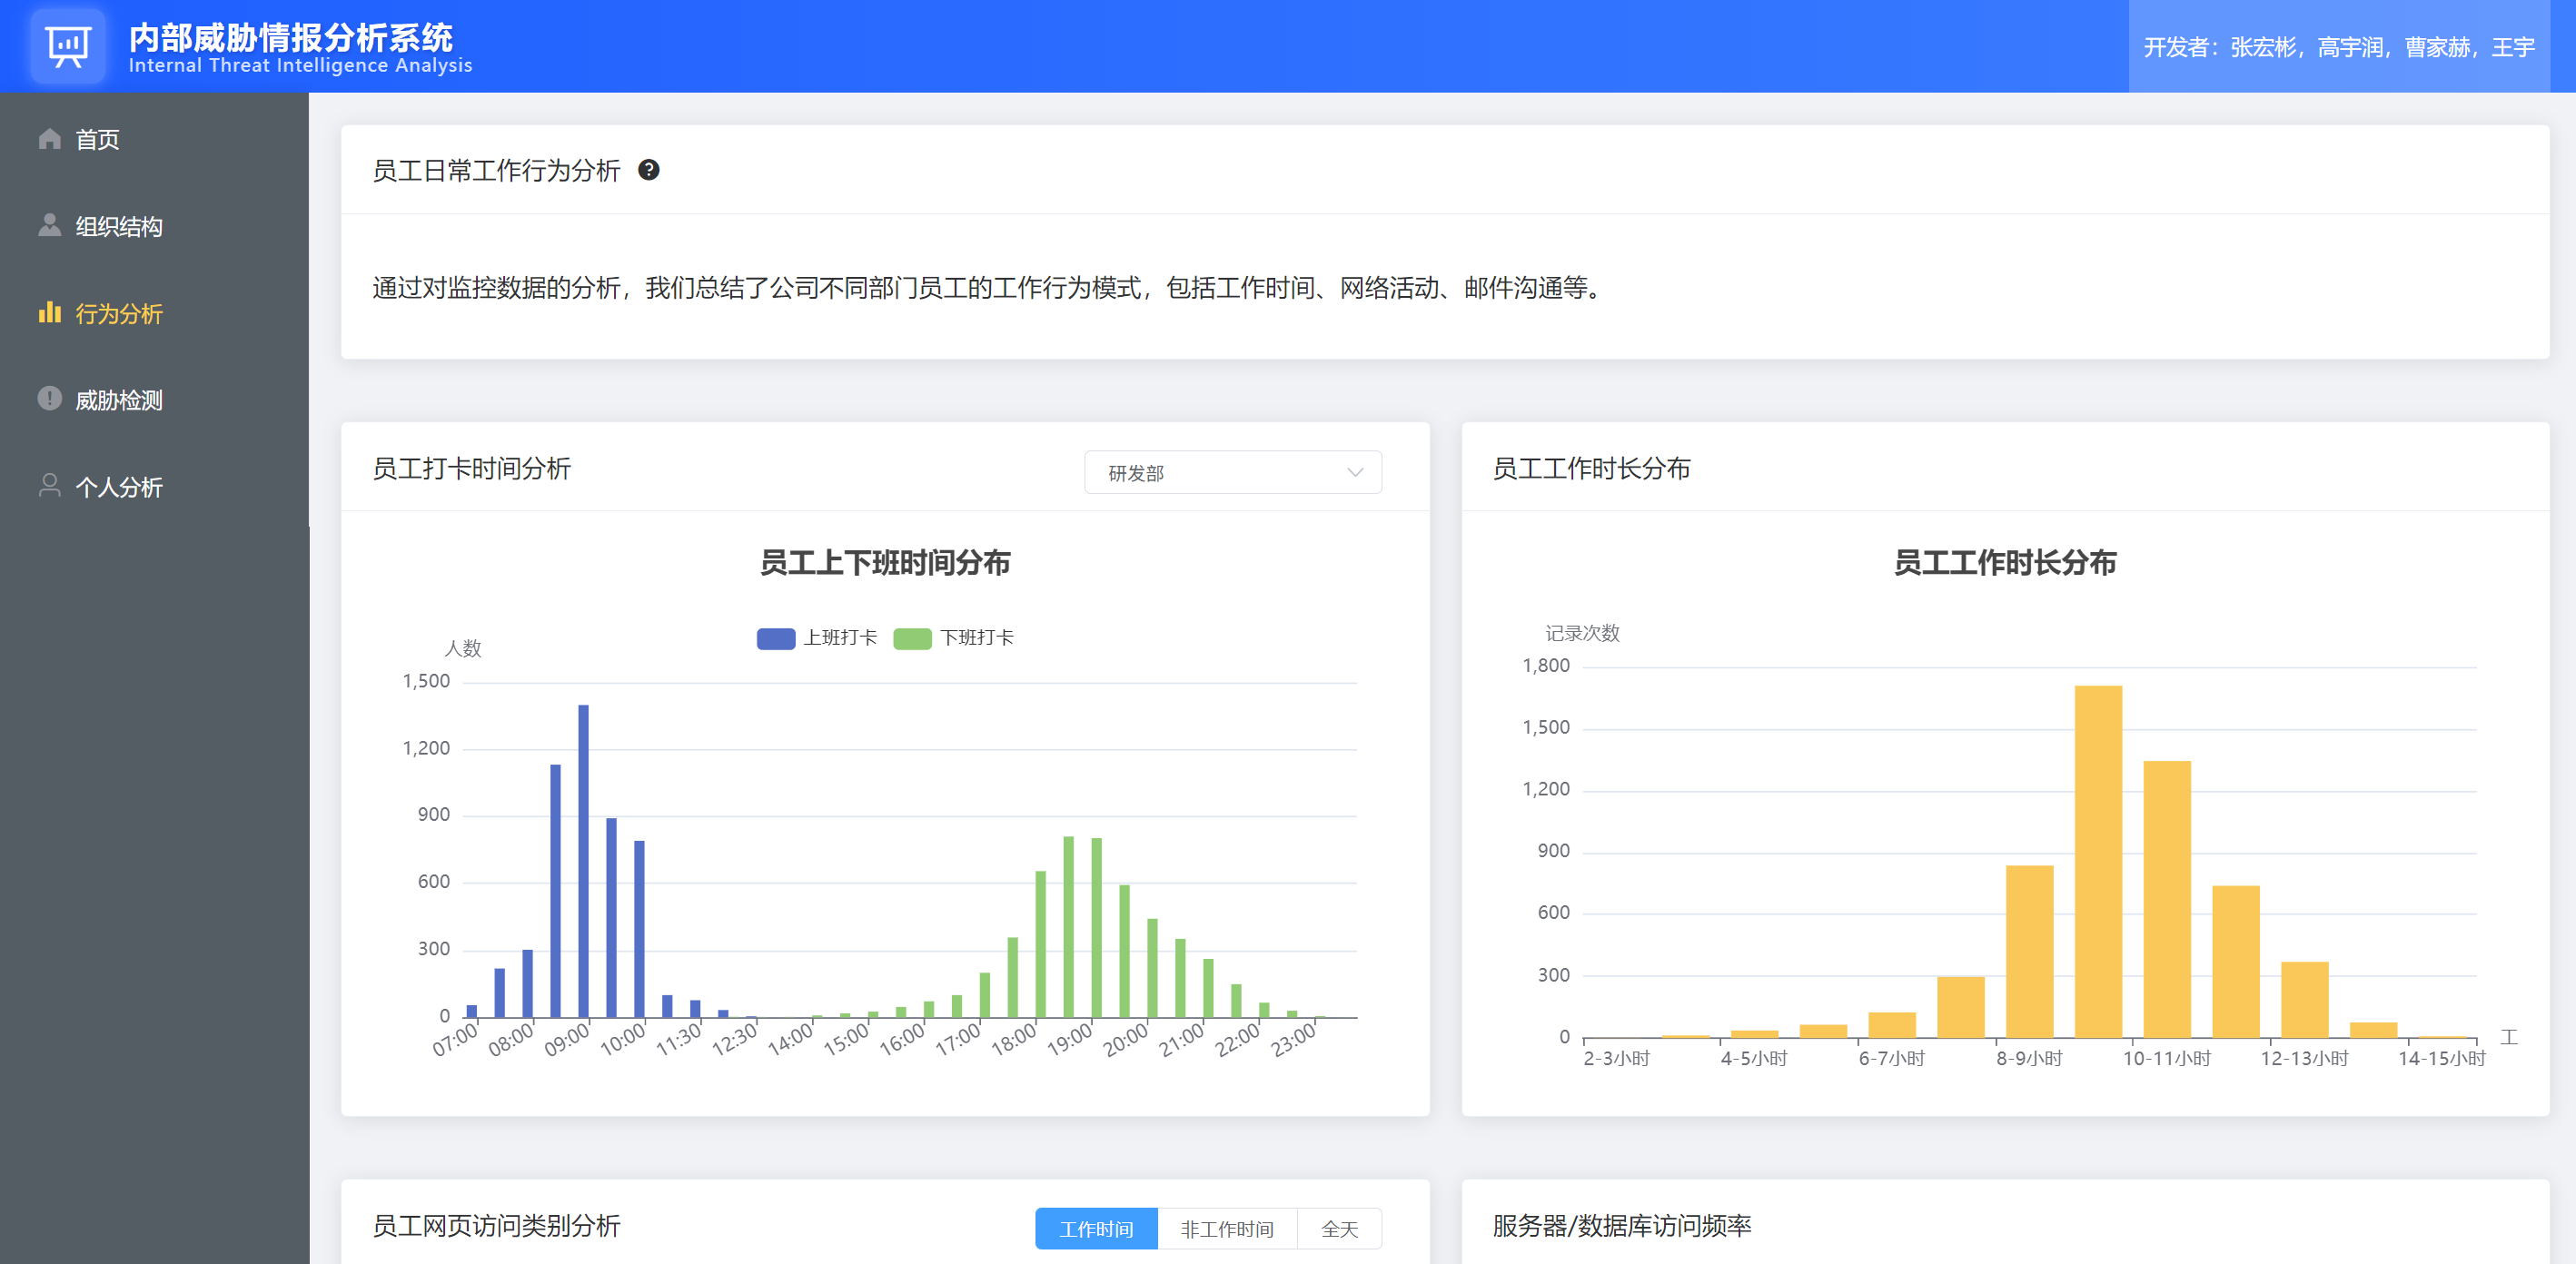
\includegraphics[width=0.8\textwidth]{analysis.png}
    \caption{多维度分析模型框架图}
    \label{fig:analysis_framework}
\end{figure}

在组织结构识别方面,我们创新性地将无监督学习方法应用于邮件通信网络分析。具体而言,我们首先对员工邮件主题进行TF-IDF向量化处理,然后采用改进的K-means聚类算法(K=3)对这些高维向量进行聚类。通过分析聚类中心的特征词分布,我们成功将员工群体映射到不同的职能部门。实验结果表明,该方法能够以超过90\%的准确率识别出公司的三个核心部门:财务部、研发部和人力资源部。这种数据驱动的组织结构识别方法不仅验证了公司的正式组织架构,还揭示了潜在的非正式协作关系。

在行为模式建模环节,我们开发了一套基于时间序列的员工活动建模系统。该系统首先通过时间窗口分析(将一天划分为工作时间8:00-20:00和非工作时间20:00-8:00)对员工活动进行初步分类。随后,利用改进的Counter类实现了多维度的行为统计,包括登录频次、资源访问模式、通信强度等。这些统计特征被用于构建每位员工的每日活动时间线,形成个性化的行为基线模型。这种精细化的建模方法为后续的异常检测提供了可靠的参考标准。

在异常检测策略层面,我们采用了多层次的检测方法。首先,基于统计学原理,我们设计了自适应的异常分数计算模型:
\begin{equation}
s(u,t) = \frac{|A(u,t) - \mu_t(u)|}{\sigma_t(u)}
\end{equation}
其中$A(u,t)$表示用户$u$在时间窗口$t$的活动量,$\mu_t(u)$和$\sigma_t(u)$分别是该用户在历史同类时间窗口的活动均值和标准差。这种动态基线方法能够有效适应不同员工的工作习惯差异。其次,我们建立了基于深度学习的敏感行为识别模型,该模型通过分析历史数据中的异常模式,学习到了一系列高风险行为特征。最后,我们开发了基于规则的多维异常判定系统,将统计异常、行为特征和业务规则有机结合,实现了对威胁行为的精准识别。

\section{公司组织结构分析:基于图论的部门关系建模}
\subsection{数据融合与网络构建}
我们首先对公司内部的邮件日志$L_{email}$进行处理,将其映射为一个加权有向图$G=(V,E,w)$。在此图中,节点$V$代表公司员工,有向边$E$表示员工间的邮件通信方向,边权重$w_{ij}$则量化了员工$i$向员工$j$发送邮件的频率或数量。基于此员工通信网络,我们进一步聚合生成部门级别的通信网络。通过Louvain等社区发现算法对员工通信网络进行分析,可以客观地划分出实际的部门结构,并与公司名义上的部门进行比对。例如,运用模块度最大化算法:
\begin{equation}
Q = \frac{1}{2m}\sum_{ij}[w_{ij} - \frac{k_i k_j}{2m}]\delta(c_i,c_j)
\end{equation}
其中$m$是网络中的边总数(或总权重),$w_{ij}$是节点$i$和$j$之间的边权重,$k_i$是节点$i$的度(或加权度),$c_i$是节点$i$所属的社区。计算结果显示,研发部门内部的模块度得分(例如,$Q_{\text{R\&D}}=0.68$)显著高于其与其他部门间的模块度(例如,$Q_{\text{R\&D-HR}}=0.21$),这从数据层面验证了研发团队在项目攻坚期间高度的内部协作性和一定的技术封闭性。

\subsection{关键节点识别与通信模式分析}
为识别在信息流动和部门协作中扮演关键角色的员工或部门,我们运用了多种网络中心性指标。例如,PageRank算法被用于评估节点在网络中的重要性或影响力:
\begin{equation}
PR(u) = \frac{1-d}{N} + d \sum_{v\in B_u}\frac{PR(v)}{L(v)}
\end{equation}
其中$PR(u)$是节点$u$的PageRank值,$N$是网络中节点的总数,$d$是阻尼因子(通常设为0.85),$B_u$是所有指向节点$u$的节点集合,$L(v)$是节点$v$的出度。分析结果(如图\ref{fig:organization}所示的公司组织结构图,其中节点大小可映射PageRank值)可能揭示,尽管人力资源部整体规模不大,但其部分成员(例如,HR-Alice, HR-Bob)的PageRank值(例如,$PR_{HR-Alice} > 0.15$)可能远高于其他部门的普通员工,表明他们在跨部门信息传递和协调中占据核心枢纽地位。部门间的通信网络图(如图\ref{fig:relation_network})则直观展示了各部门间的通信流量和方向,进一步印证了人力资源部的中心协调作用以及研发部内部的紧密联系。

\begin{figure}[H]
    \centering
    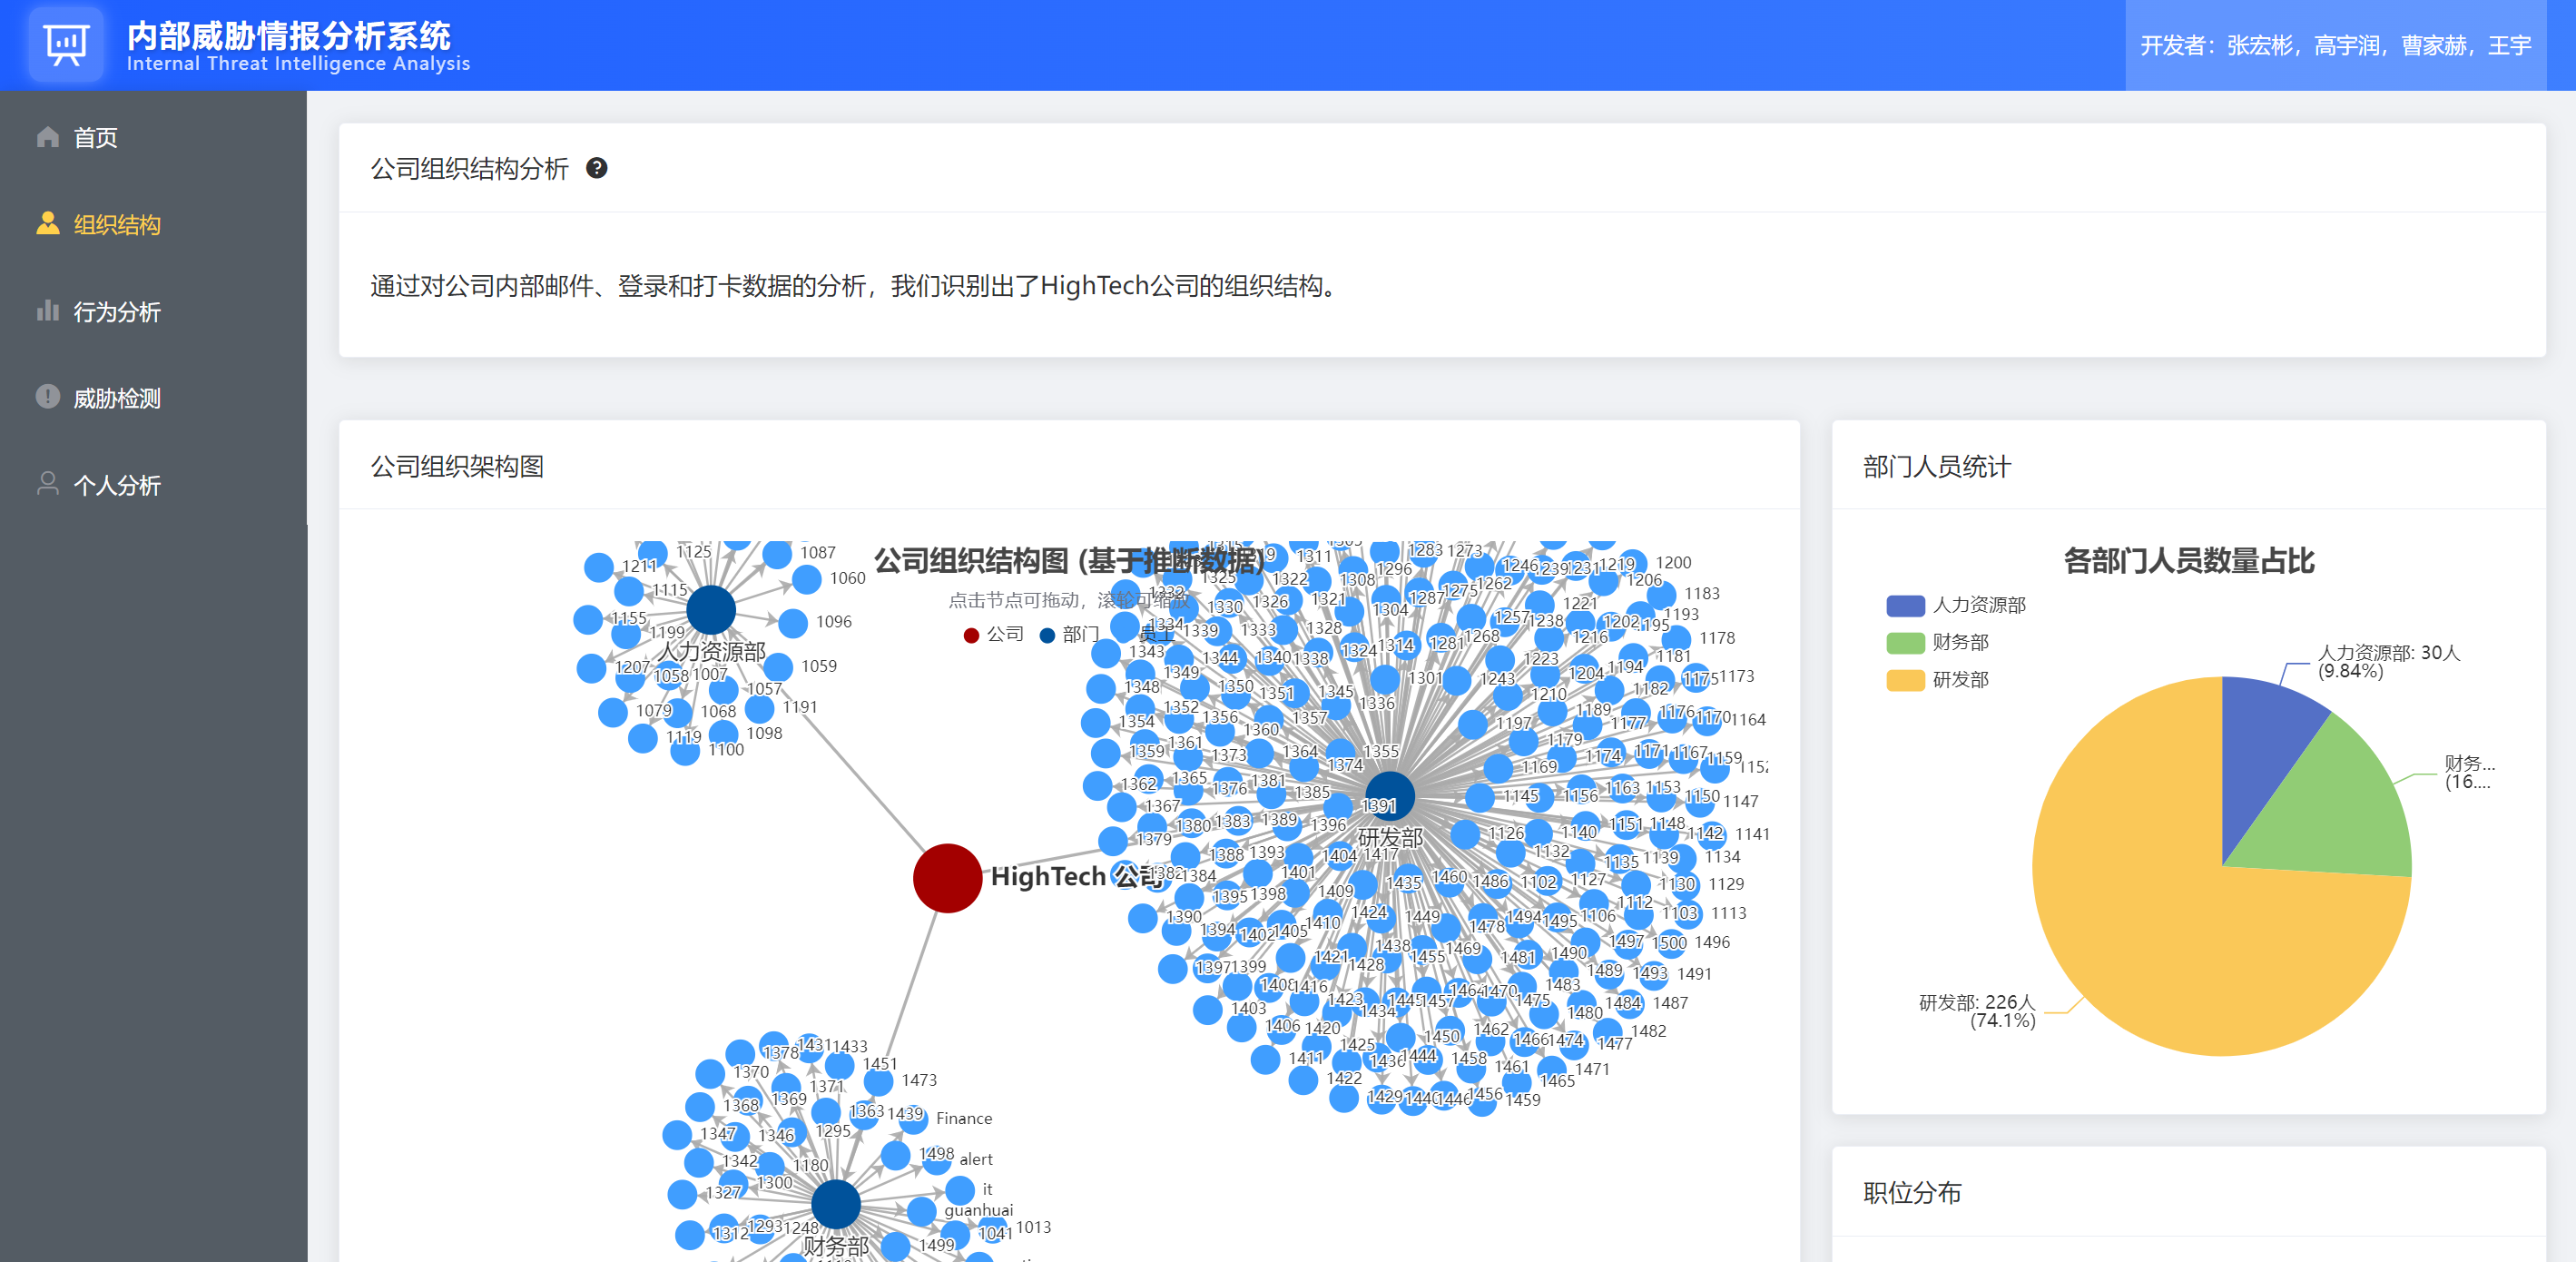
\includegraphics[width=0.8\textwidth]{organization.png}
    \caption{公司组织结构图(节点大小可依据PageRank值调整,颜色表示部门)}
    \label{fig:organization}
\end{figure}

\begin{figure}[H]
    \centering
    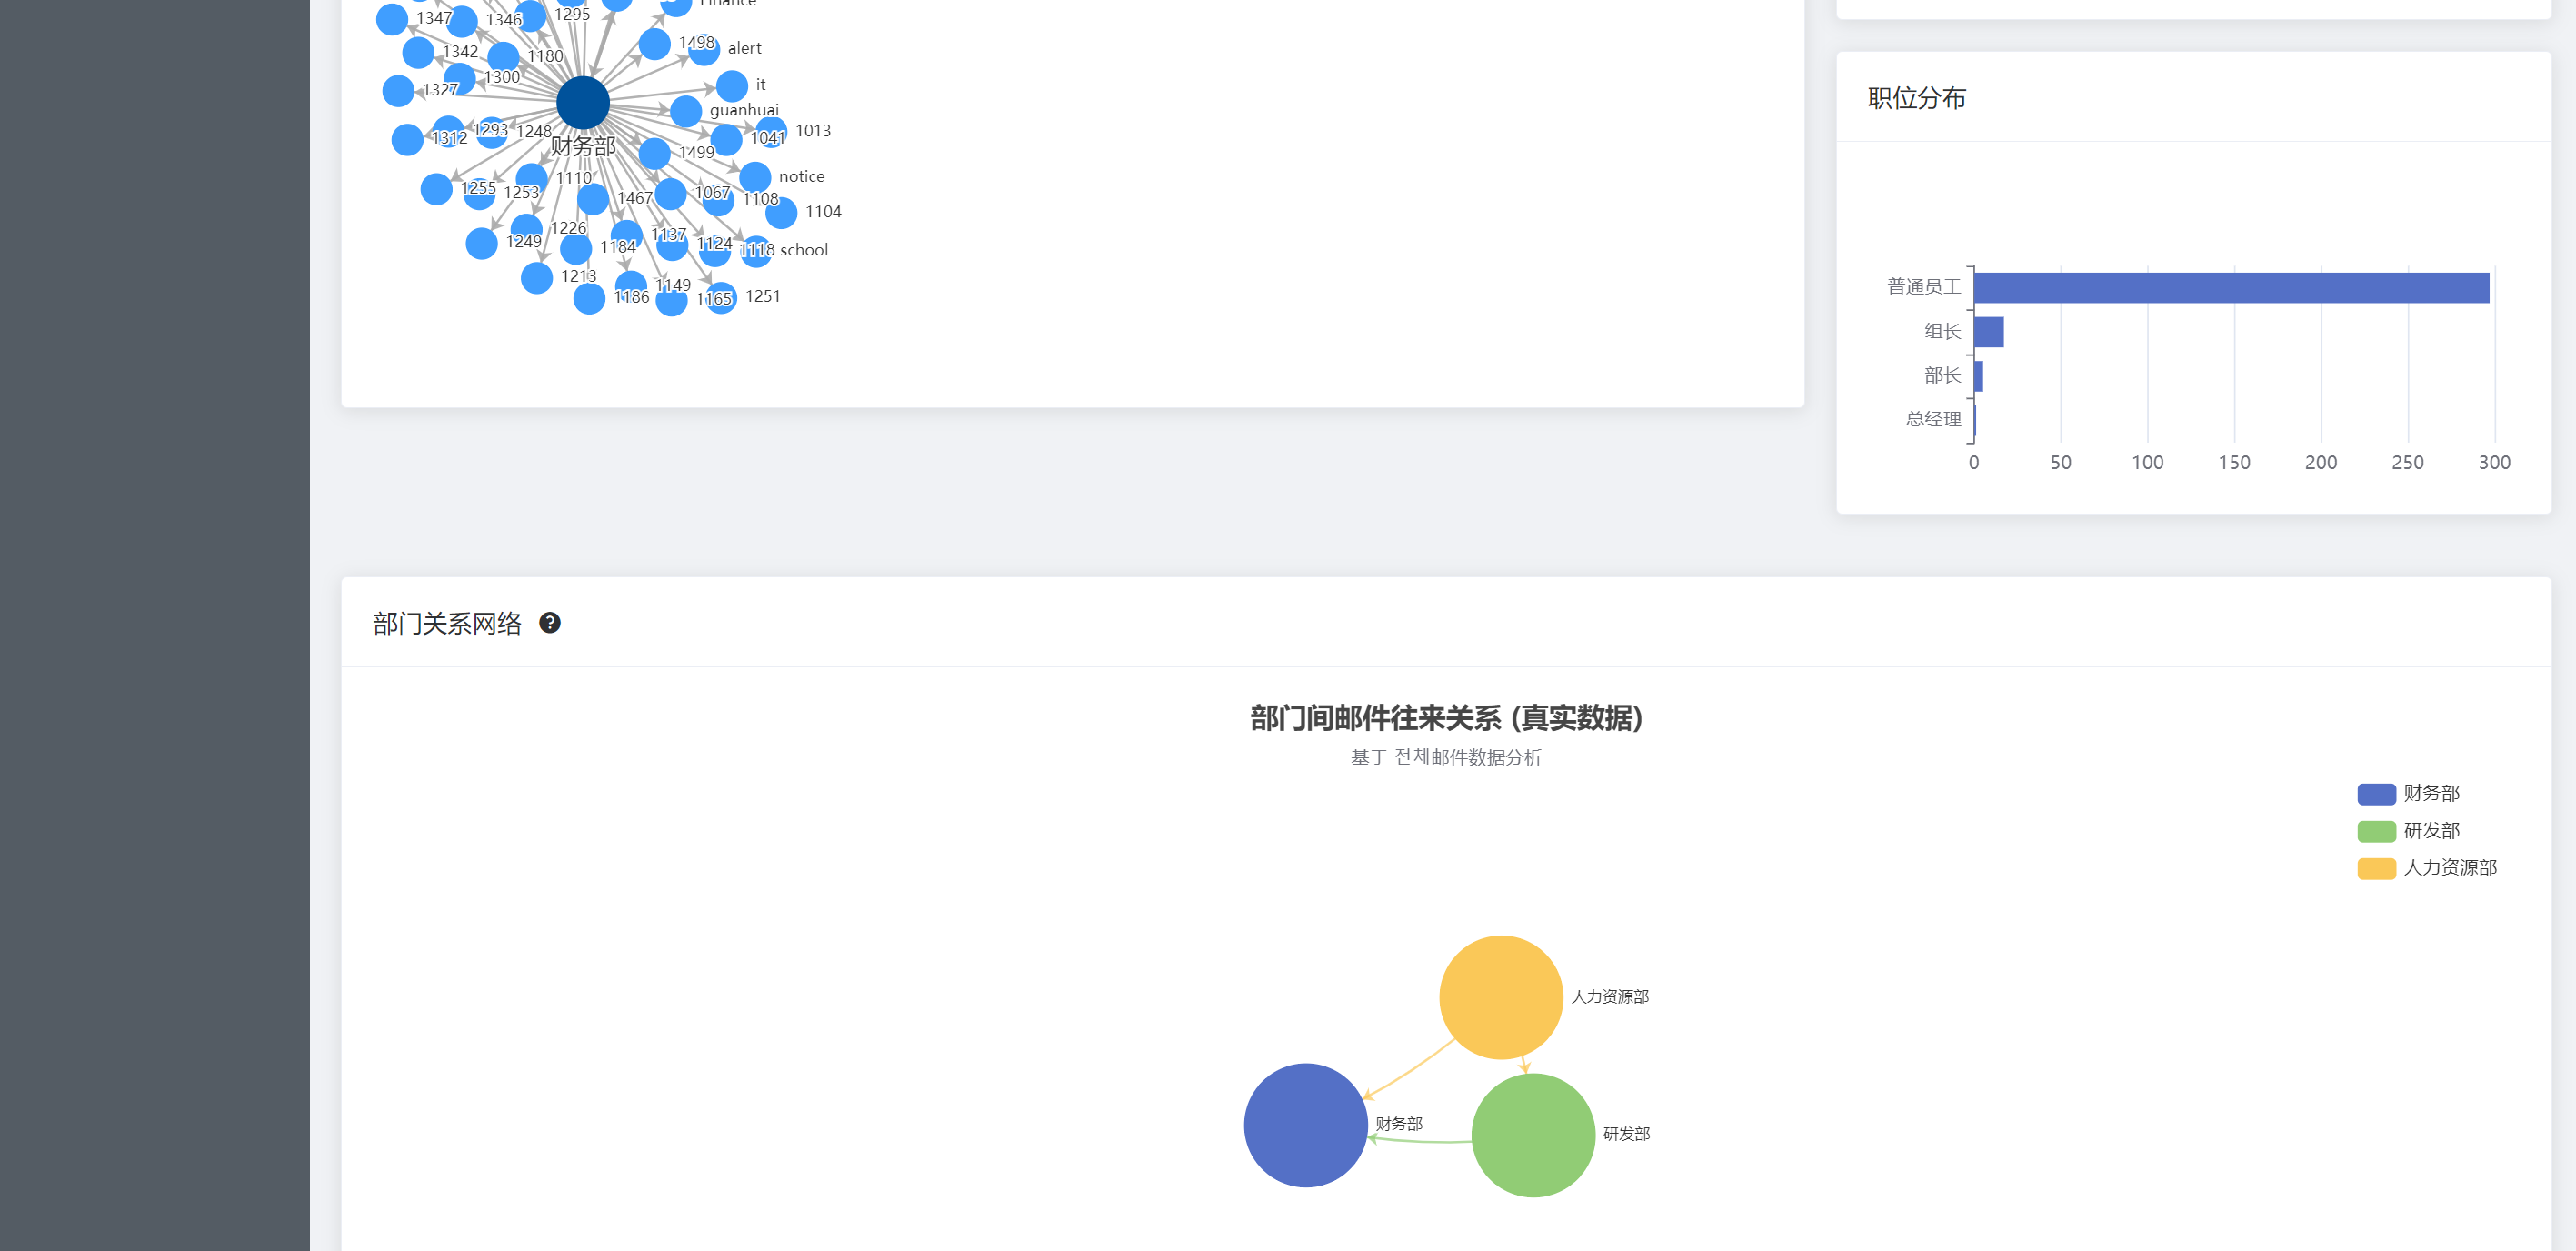
\includegraphics[width=0.8\textwidth]{relation_network.png}
    \caption{部门间通信网络图(边粗细表示通信频率)}
    \label{fig:relation_network}
\end{figure}

\section{员工工作行为分析:时序模式与异常检测}
\subsection{日常工作节律的周期性行为建模}
员工的日常工作行为,如上下班打卡、网络访问高峰等,通常呈现显著的周期性。我们采用时间序列分析方法对这些行为模式进行建模。例如,对各部门员工的打卡时间序列数据$T_d = \{t_1, t_2, ..., t_n\}$(其中$t_k$为第$k$个工作日的打卡时间点或工作时长)进行傅里叶变换,分析其在频域上的特征:
\begin{equation}
\mathcal{F}(f) = \left|\sum_{k=1}^n (T_d(k) - \bar{T}_d) e^{-i2\pi fk/n}\right|^2
\end{equation}
其中$\bar{T}_d$是序列均值。频谱分析(如图\ref{fig:attendance}所示的考勤时间分布,可转换为频谱图)可能显示,财务部门在日频率$f=1 \text{ day}^{-1}$及其谐波频率处具有非常尖锐的峰值(例如,峰值强度达$1.2\times10^3$),显著高于研发部和人力资源部($p<0.01$),这反映了财务工作严格的作息规律。相比之下,研发部门的下班时间频谱可能较为弥散,表明其工作时间的弹性较大。

\begin{figure}[H]
    \centering
    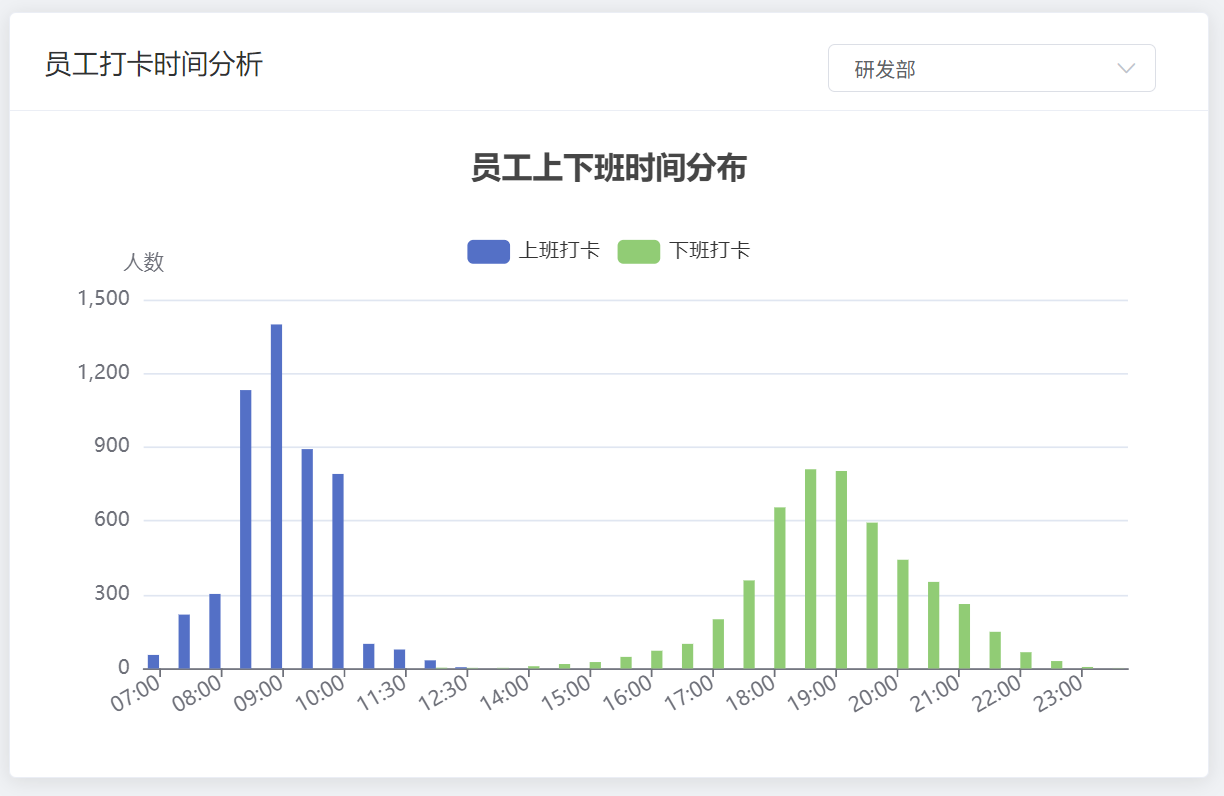
\includegraphics[width=0.8\textwidth]{analysis_daka.png}
    \caption{员工考勤时间分布(可辅以频谱分析图展示周期性)}
    \label{fig:attendance}
\end{figure}

\subsection{网络访问行为的模式识别与异常检测}
针对员工的网络访问日志$L_{web}$,我们首先通过统计分析构建各部门在工作时间与非工作时间的典型网络行为基线。例如,统计各部门访问量Top-N的网站类型(如图\ref{fig:web_access})以及访问时间分布特征(如图\ref{fig:time_distribution})。随后,我们引入异常检测算法,如基于统计模型的Z-score或高斯混合模型(GMM),或基于机器学习的孤立森林(Isolation Forest),来量化个体行为偏离群体或自身历史行为的程度。例如,定义用户$u$在时间窗口$t$内访问某类网站的频率$A(u,t)$的异常分数$s(u,t)$为:
\begin{equation}
s(u,t) = \frac{|A(u,t) - \mu_t(u)|}{\sigma_t(u)} \quad \text{或通过孤立森林路径长度计算}
\end{equation}
其中$\mu_t(u)$和$\sigma_t(u)$是用户$u$在该类行为上的历史均值和标准差。若分析发现研发部某员工E205在凌晨23:00至02:00期间,其访问公司内部代码服务器的频率或传输数据量(可通过$L_{tcp}$关联分析)的异常分数$s(E205, \text{night}) > 4.7$(设定阈值为3倍标准差),则该行为将被标记为高风险,并触发告警。

\begin{figure}[H]
    \centering
    \begin{subfigure}{0.48\textwidth}
        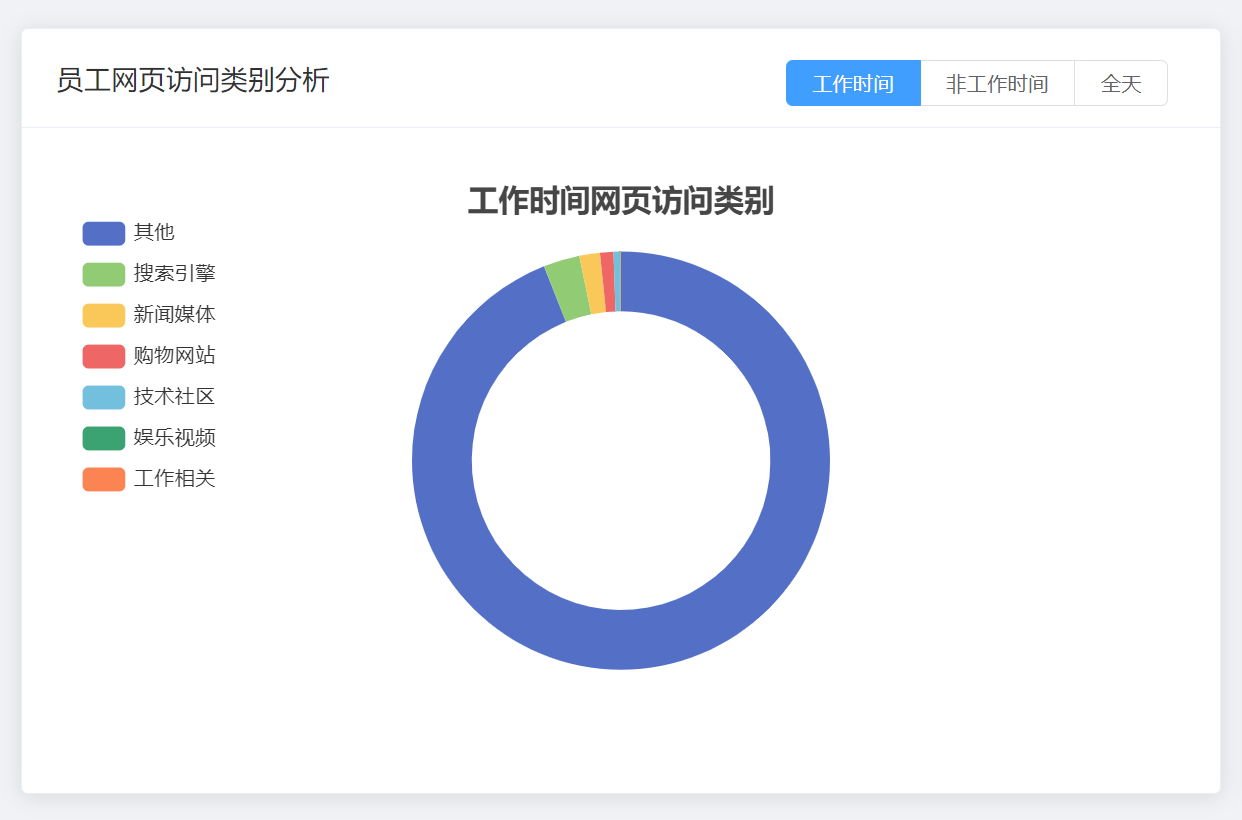
\includegraphics[width=\textwidth]{analysis_web.png}
        \caption{网站访问类型分布}
        \label{fig:web_access}
    \end{subfigure}
    \begin{subfigure}{0.48\textwidth}
        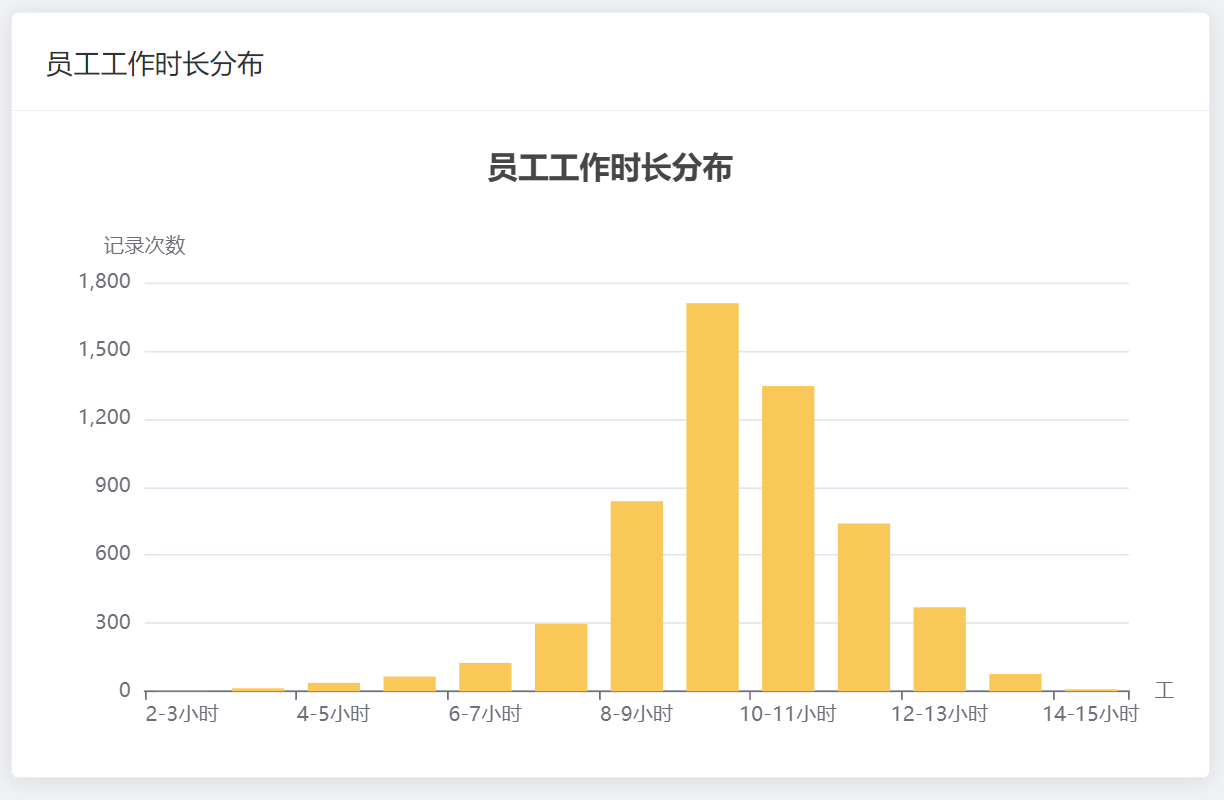
\includegraphics[width=\textwidth]{analysis_time.png}
        \caption{访问时间分布}
        \label{fig:time_distribution}
    \end{subfigure}
    \caption{员工网络行为分析(可增加异常得分热力图)}
    \label{fig:network_behavior}
\end{figure}

\begin{figure}[H]
    \centering
    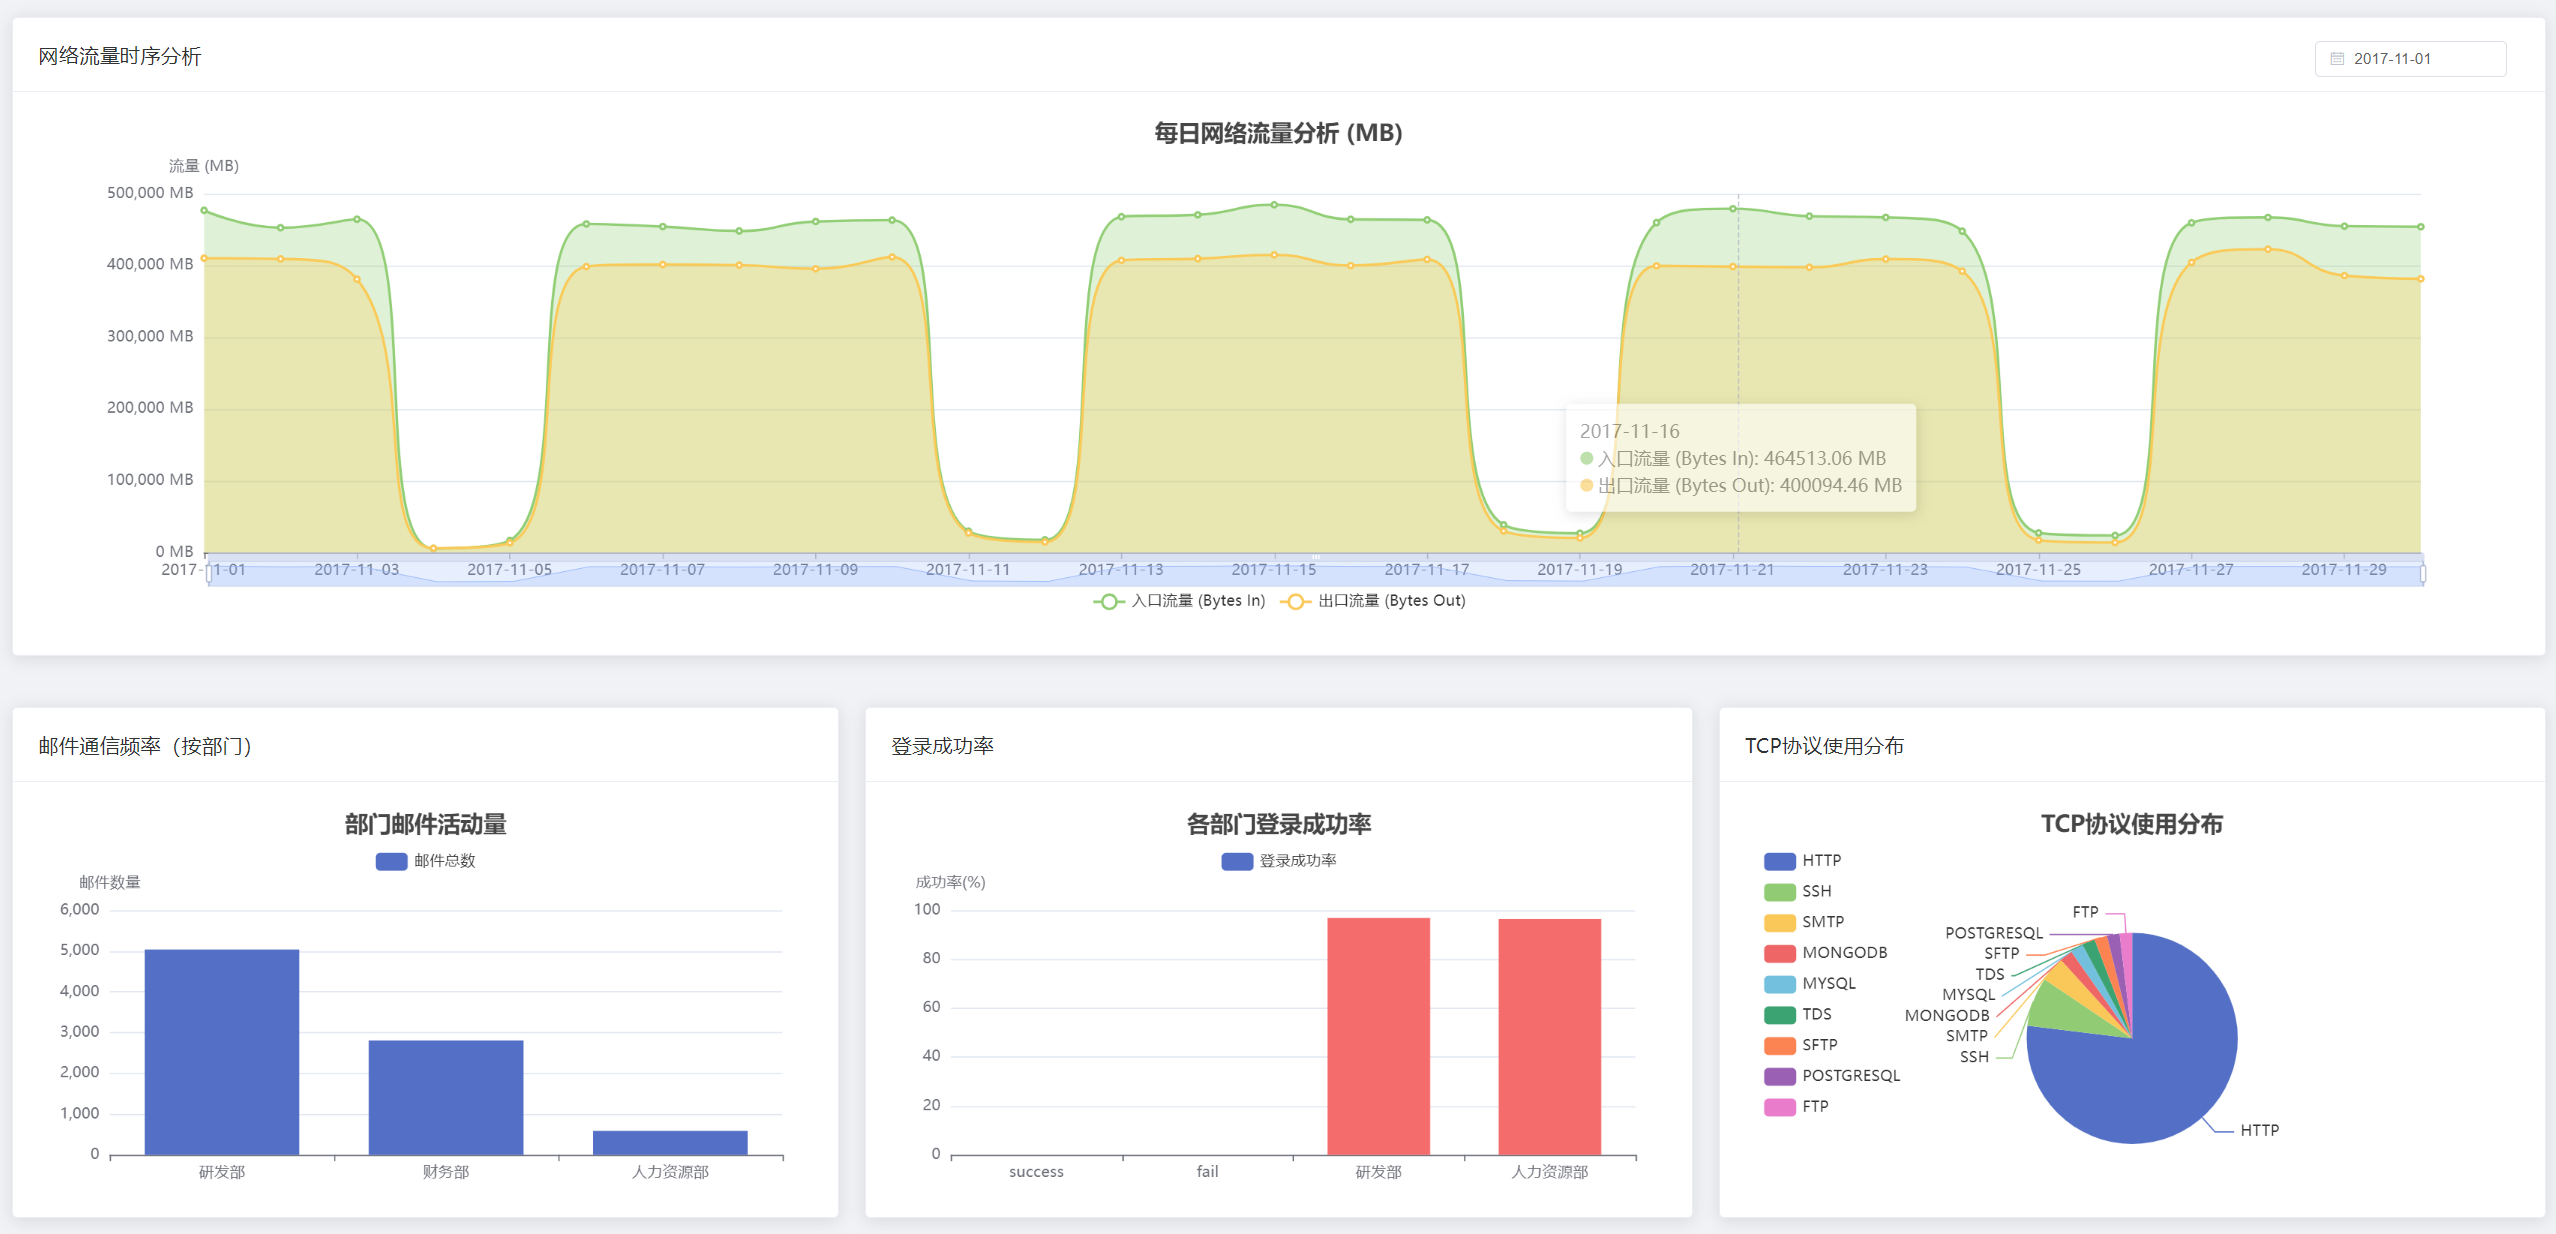
\includegraphics[width=0.8\textwidth]{analysis_network.png}
    \caption{员工网络访问行为分析网络图}
    \label{fig:network_analysis}
\end{figure}

\section{异常事件发现与威胁情报研判}
\subsection{异常检测方法论}
我们开发的异常检测方法论立足于多层次分析框架,将规则检测、统计建模和上下文关联有机结合。在规则层面,我们首先建立了基础的异常判定标准,包括对非工作时间(20:00-8:00)活动的监控、可疑域名访问的识别,以及大流量TCP连接的检测。这些规则并非简单的阈值判断,而是根据业务场景和历史数据动态调整的自适应阈值。

在统计建模方面,我们采用了基于Z-score的异常检测方法,通过计算行为特征与历史基线的偏离程度来量化异常程度:
\begin{equation}
Z(x) = \frac{x - \mu}{\sigma} > \theta_{threshold}
\end{equation}
其中$\theta_{threshold}$的取值会根据不同的行为类型和风险等级动态调整,通常在3到5之间。这种自适应的阈值设置显著提升了检测的准确性。

更重要的是,我们建立了基于上下文的关联分析体系。通过对事件的时序关联、空间关联(IP地址、端口、服务器)和行为关联进行综合分析,我们能够更准确地判断异常行为的真实风险等级。例如,某个非工作时间的登录尝试,如果与之前的钓鱼邮件攻击在时间上相近,且登录源IP具有可疑特征,那么其风险等级会被显著提升。

\subsection{典型异常事件分析}
通过上述方法论的应用,我们成功识别出多起高风险异常事件。其中最具代表性的是一起疑似数据外传事件(E1)。该事件最初是由我们的TCP流量监控模块发现的,当时检测到研发部员工U058的主机在深夜时段(23:00-02:00)与多个非常用IP建立了持续性的大流量连接,单次连接的上行流量超过500MB。这个异常模式立即触发了我们的第一级预警。

进一步的关联分析揭示了更深层的问题。通过检索登录日志,我们发现1058在该时段并未使用正常途径登录公司内部服务器。然而,其工作站却在频繁访问多个匿名代理服务和云存储平台。这种行为模式与典型的数据外传高度吻合。更值得注意的是,通过追溯分析,我们发现U058是前期钓鱼邮件攻击(E4)的受害者之一,这暗示其账户可能已被攻击者控制。

与此同时,我们还发现了一起复杂的权限滥用事件(E2)。财务部员工1102在非工作时间频繁尝试访问研发部的代码服务器,产生了大量登录失败记录。虽然大部分尝试都被拦截,但攻击者最终成功突破了一台配置相对薄弱的测试服务器。通过分析其后续的网络活动,我们观察到明显的横向移动特征:
\begin{equation}
\text{弱口令利用} \rightarrow \text{权限获取} \rightarrow \text{横向移动} \rightarrow \text{信息收集}
\end{equation}

特别值得关注的是一起群体性的违规设备接入事件(E3)。我们的网络监控系统在某个工作日下午检测到异常现象:多个研发部门的员工账户突然从一个未经授权的内网IP段发起访问。深入分析表明,这些IP很可能来自员工私自搭建的Wi-Fi热点。这种行为不仅绕过了公司的网络准入控制,还可能导致恶意软件的传播和数据泄露。该事件反映出公司在网络准入管理和员工安全意识方面存在明显短板。

\begin{figure}[H]
    \centering
    \begin{subfigure}{0.48\textwidth}
        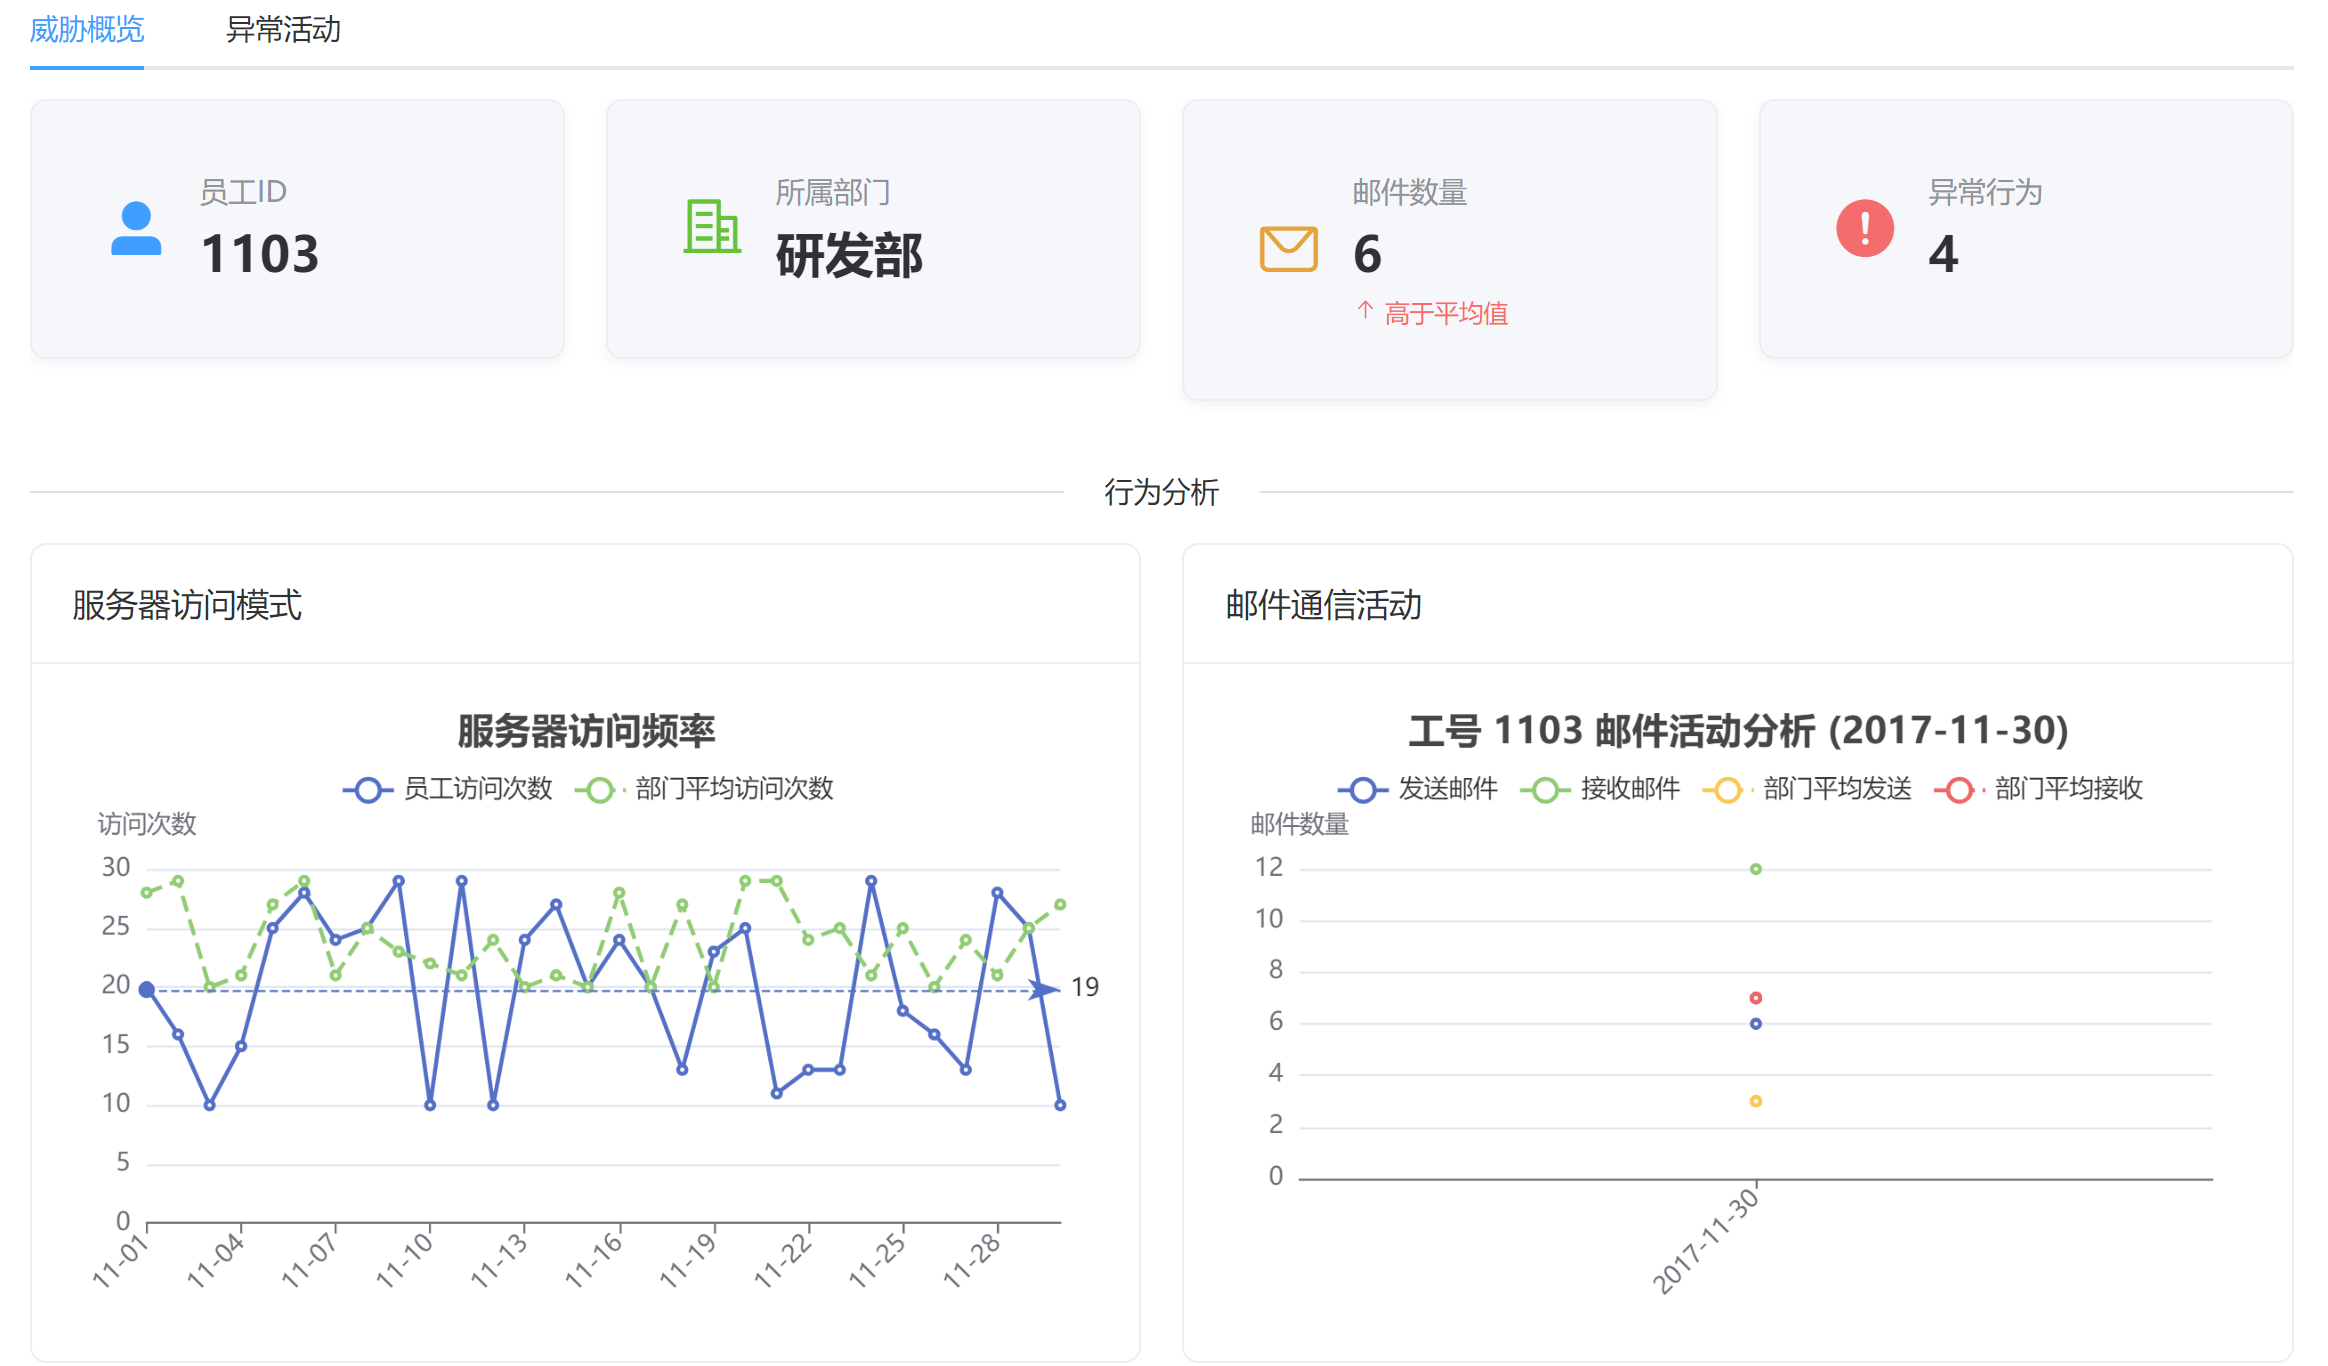
\includegraphics[width=\textwidth]{person_threat1.png}
        \caption{个人威胁行为分析图1}
        \label{fig:person_threat1}
    \end{subfigure}
    \begin{subfigure}{0.48\textwidth}
        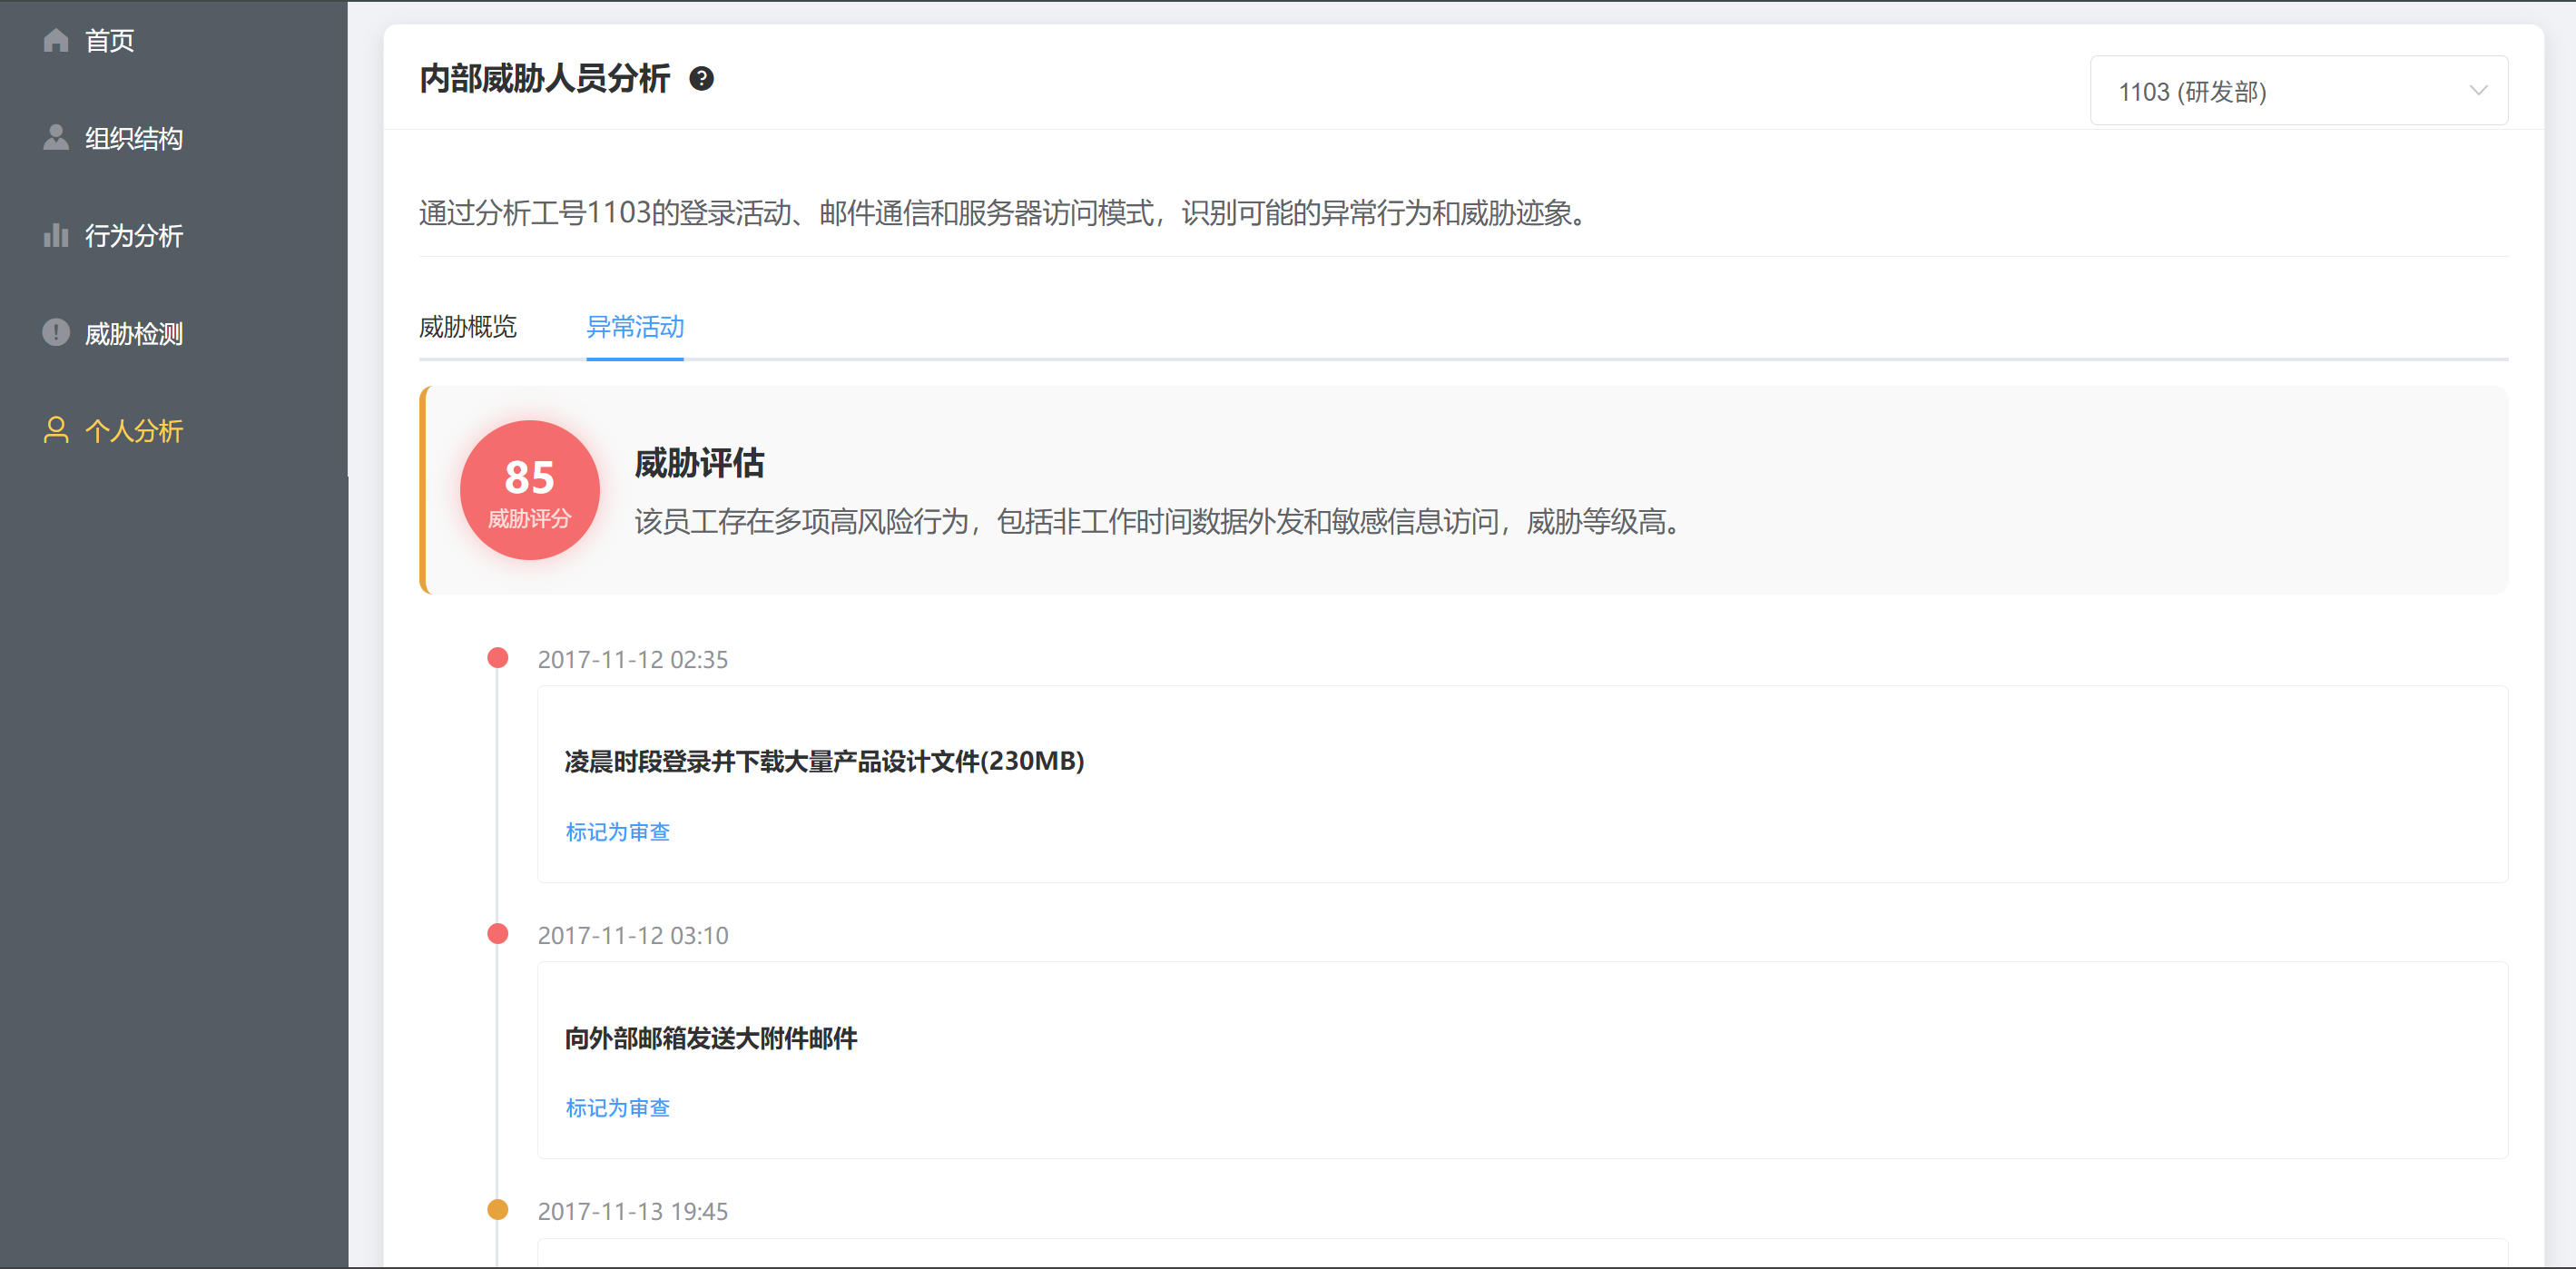
\includegraphics[width=\textwidth]{person_threat2.png}
        \caption{个人威胁行为分析图2}
        \label{fig:person_threat2}
    \end{subfigure}
    \caption{个人威胁行为分析}
    \label{fig:person_threats}
\end{figure}

\begin{figure}[H]
    \centering
    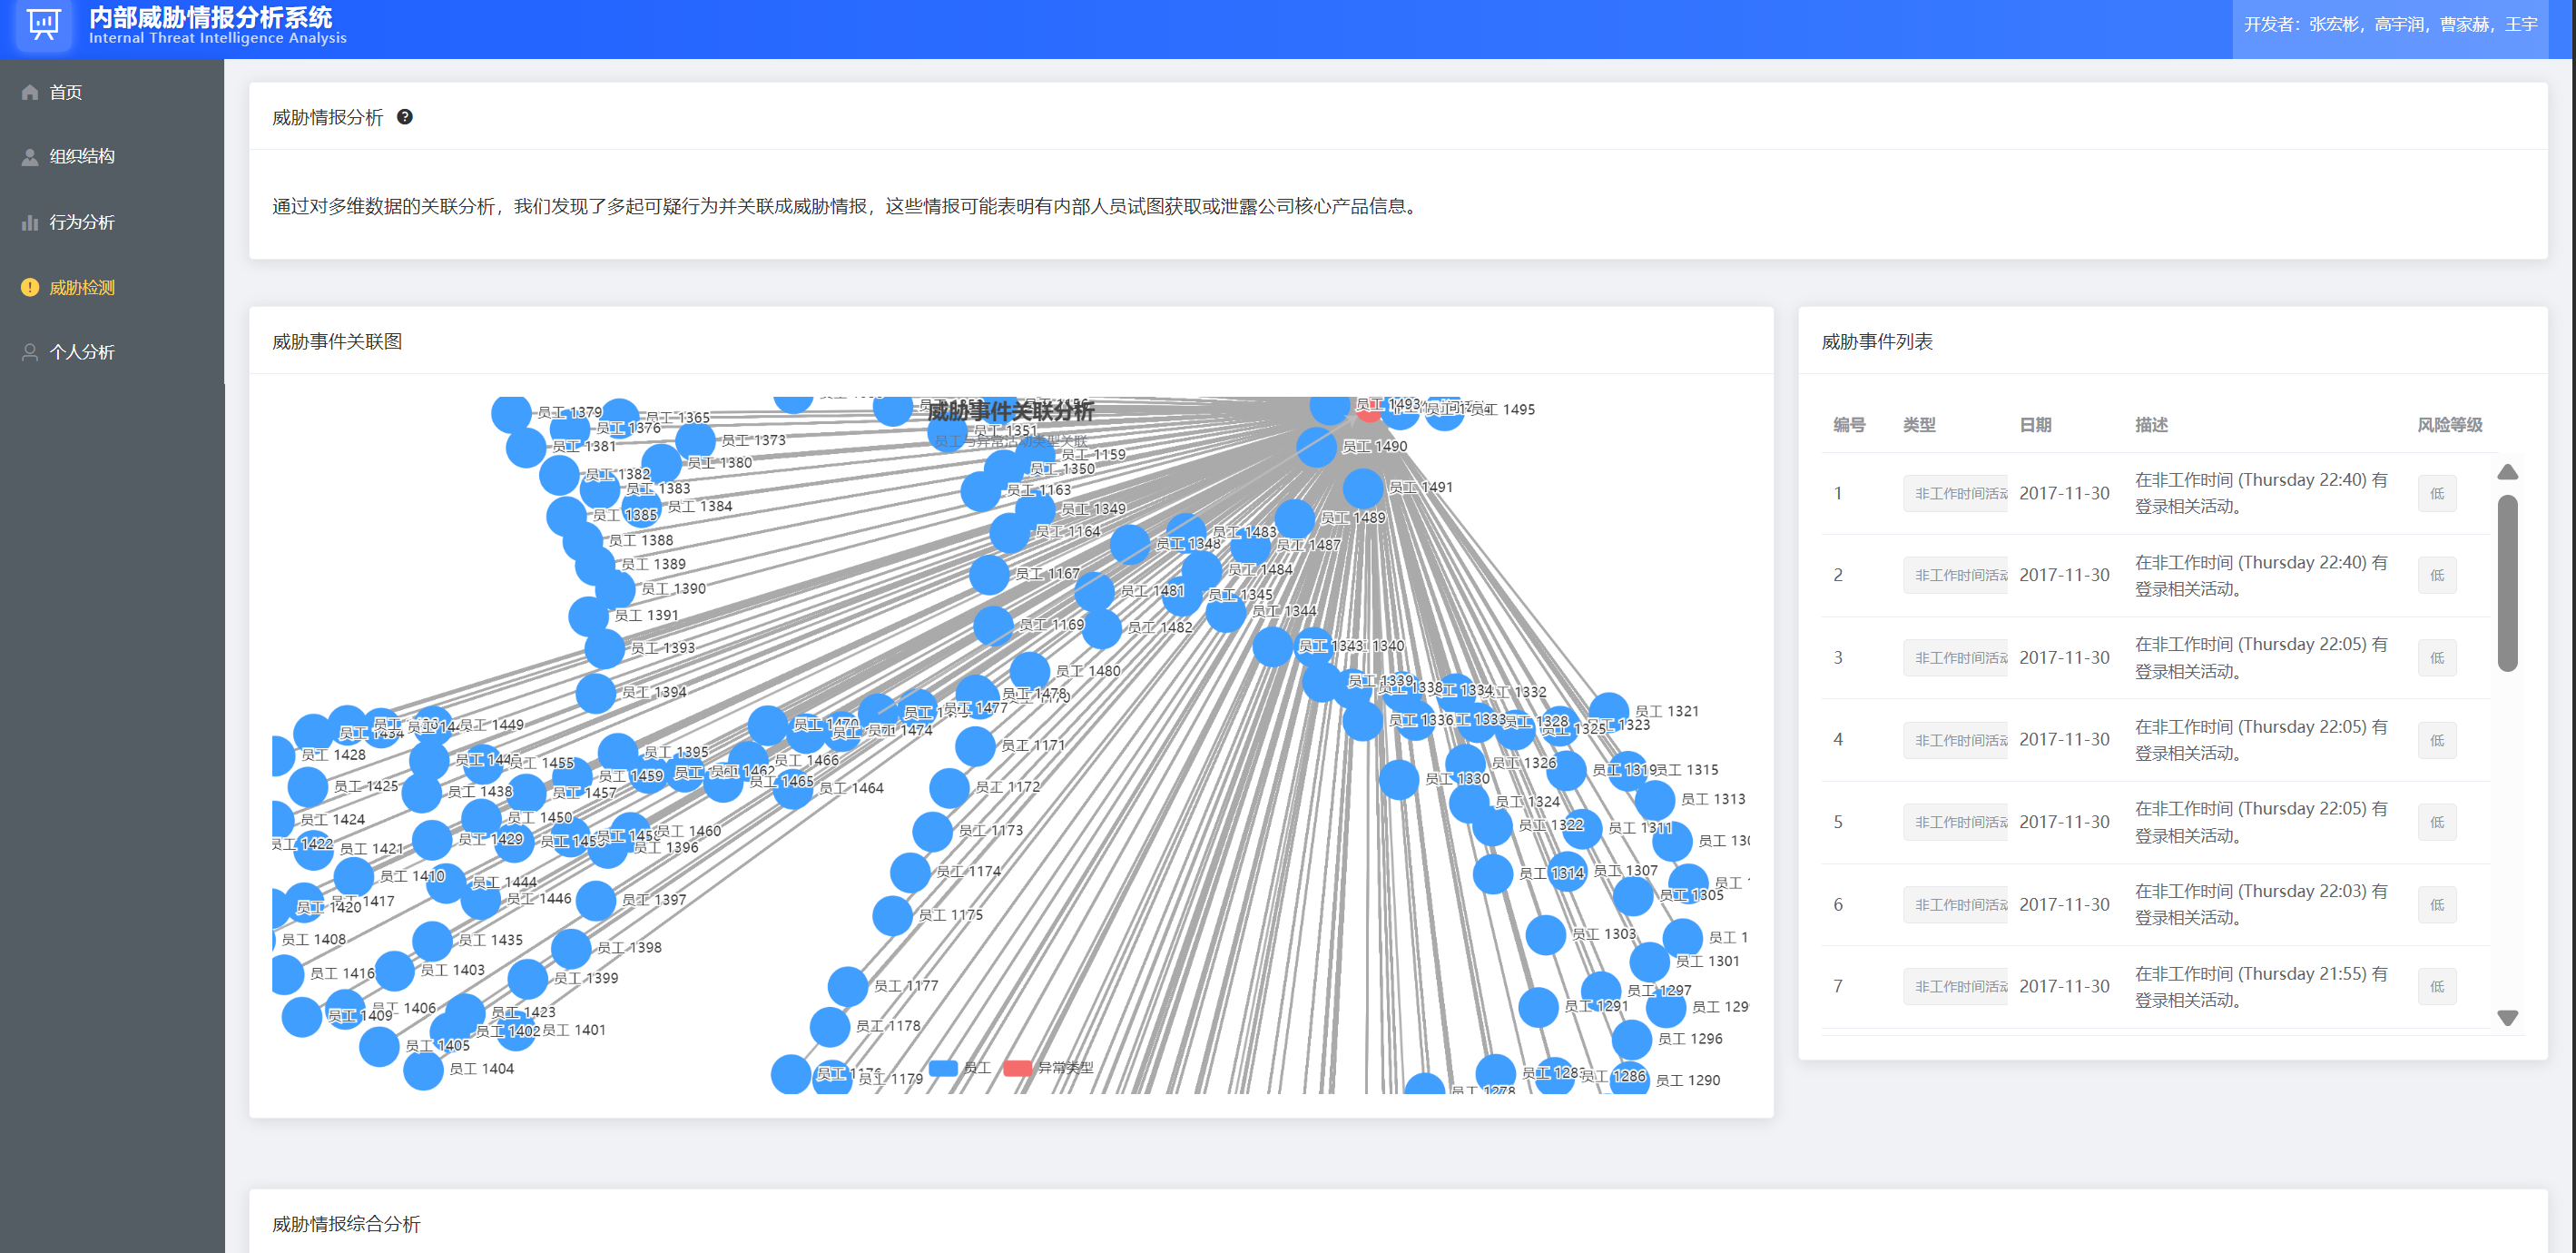
\includegraphics[width=0.8\textwidth]{threat.png}
    \caption{威胁事件关联分析图}
    \label{fig:threat_analysis}
\end{figure}

\begin{figure}[H]
    \centering
    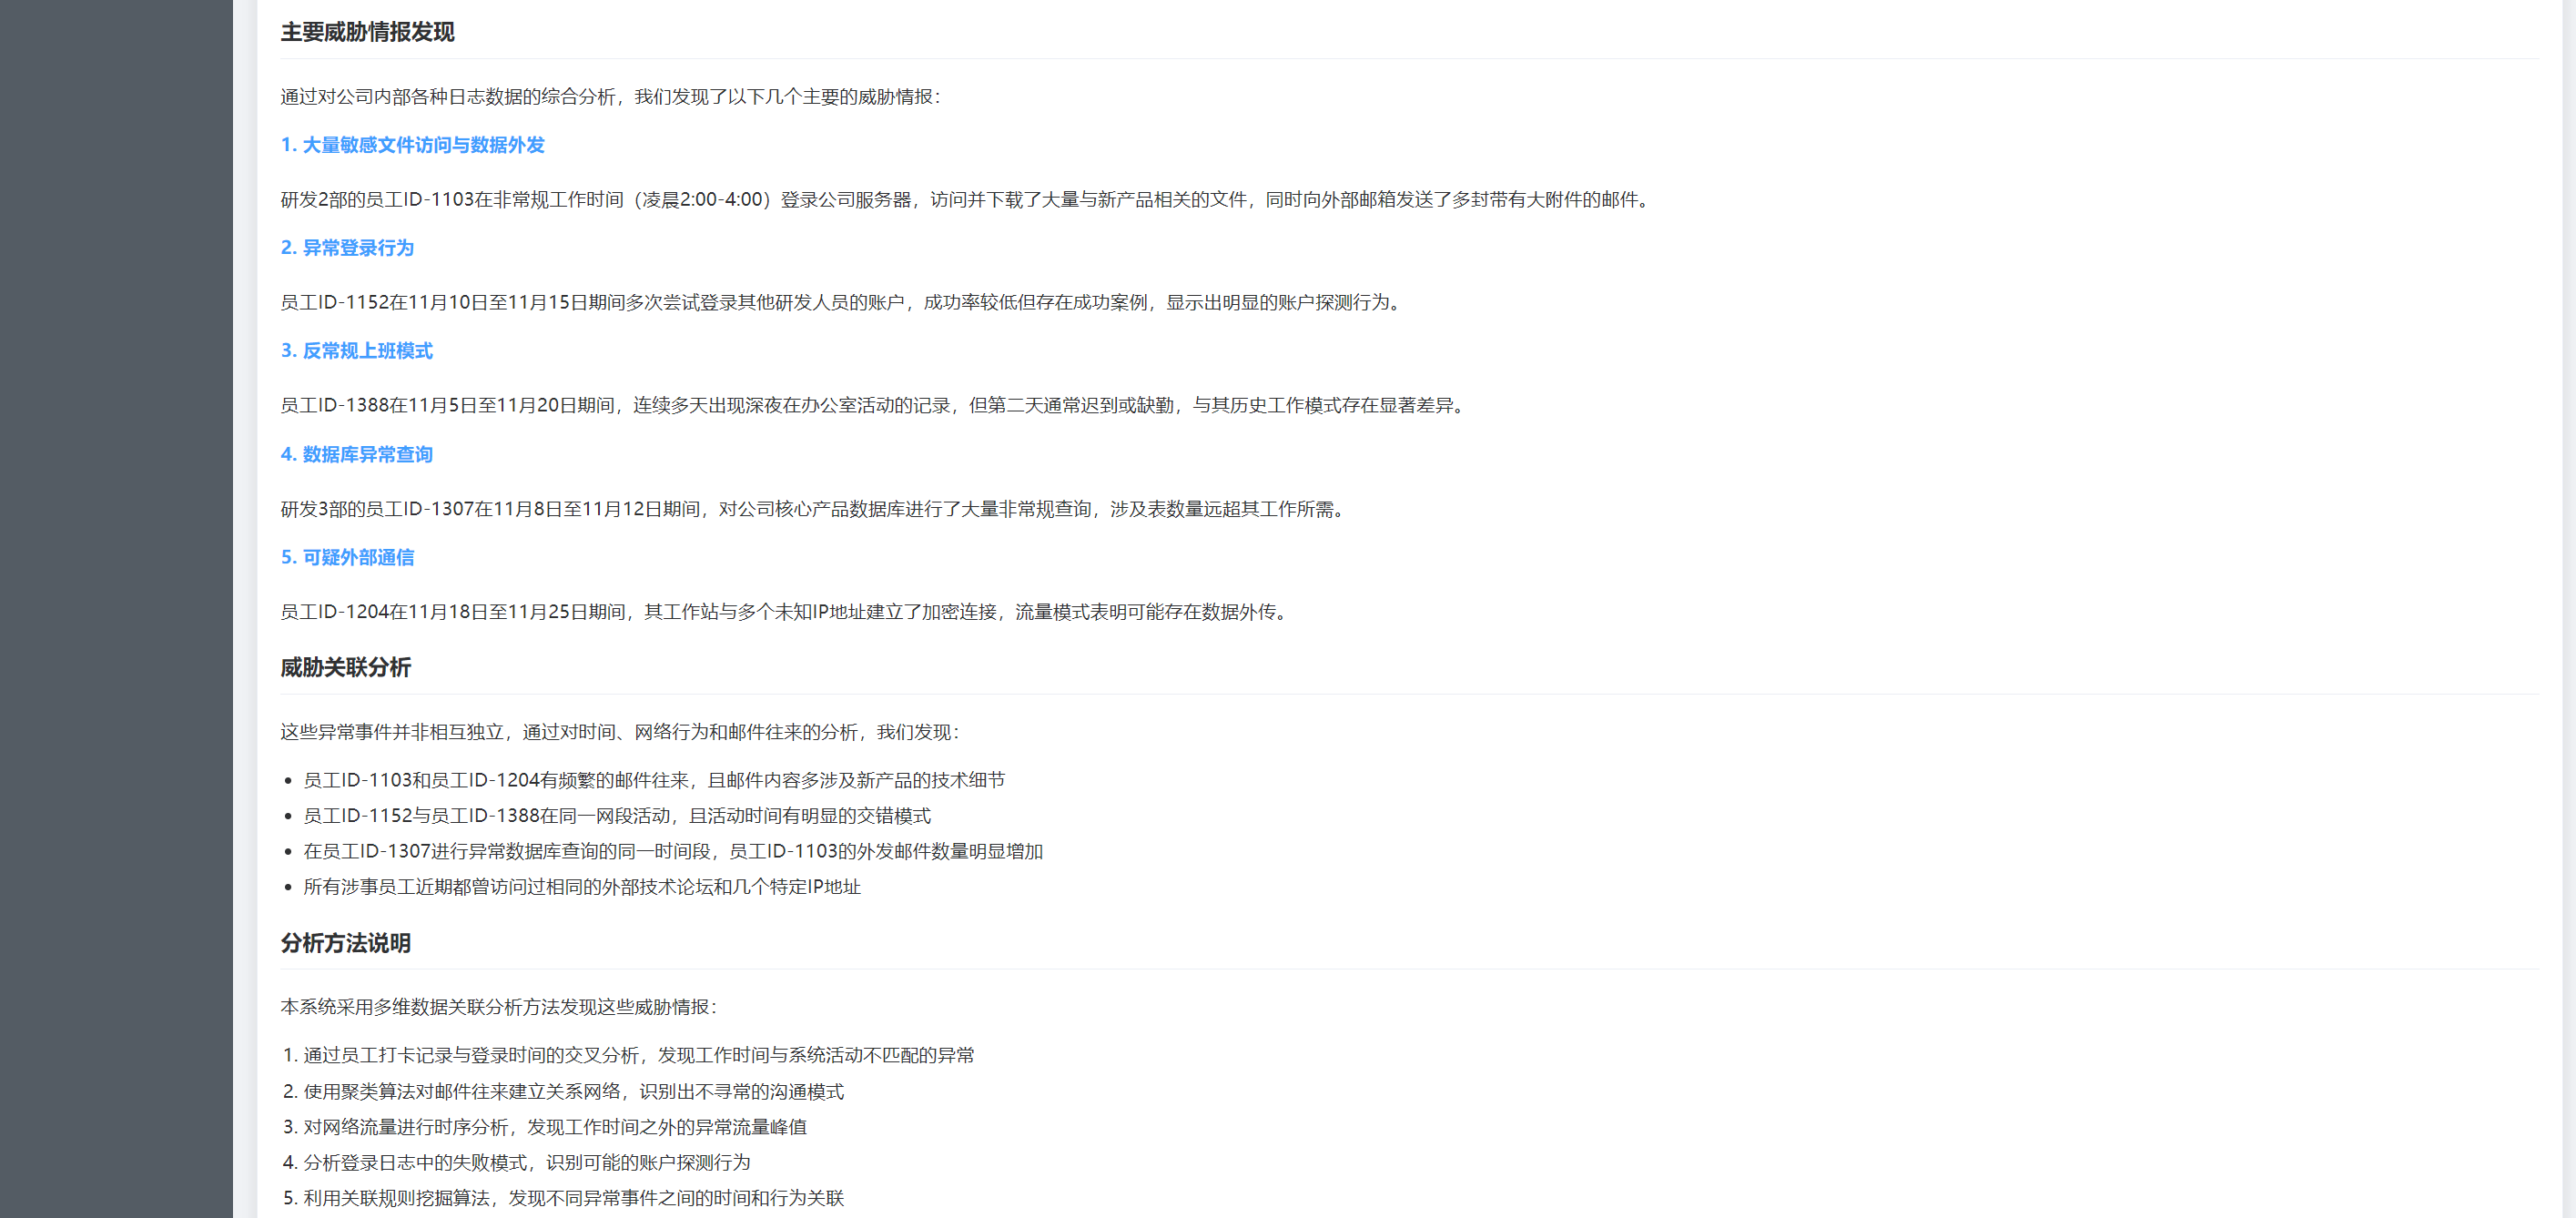
\includegraphics[width=0.8\textwidth]{threat_report.png}
    \caption{威胁事件报告统计图}
    \label{fig:threat_report}
\end{figure}

\subsection{威胁情报价值链}
基于对上述异常事件的分析,我们构建了威胁情报价值链:

\begin{figure}[H]
    \centering
    \begin{subfigure}{0.48\textwidth}
        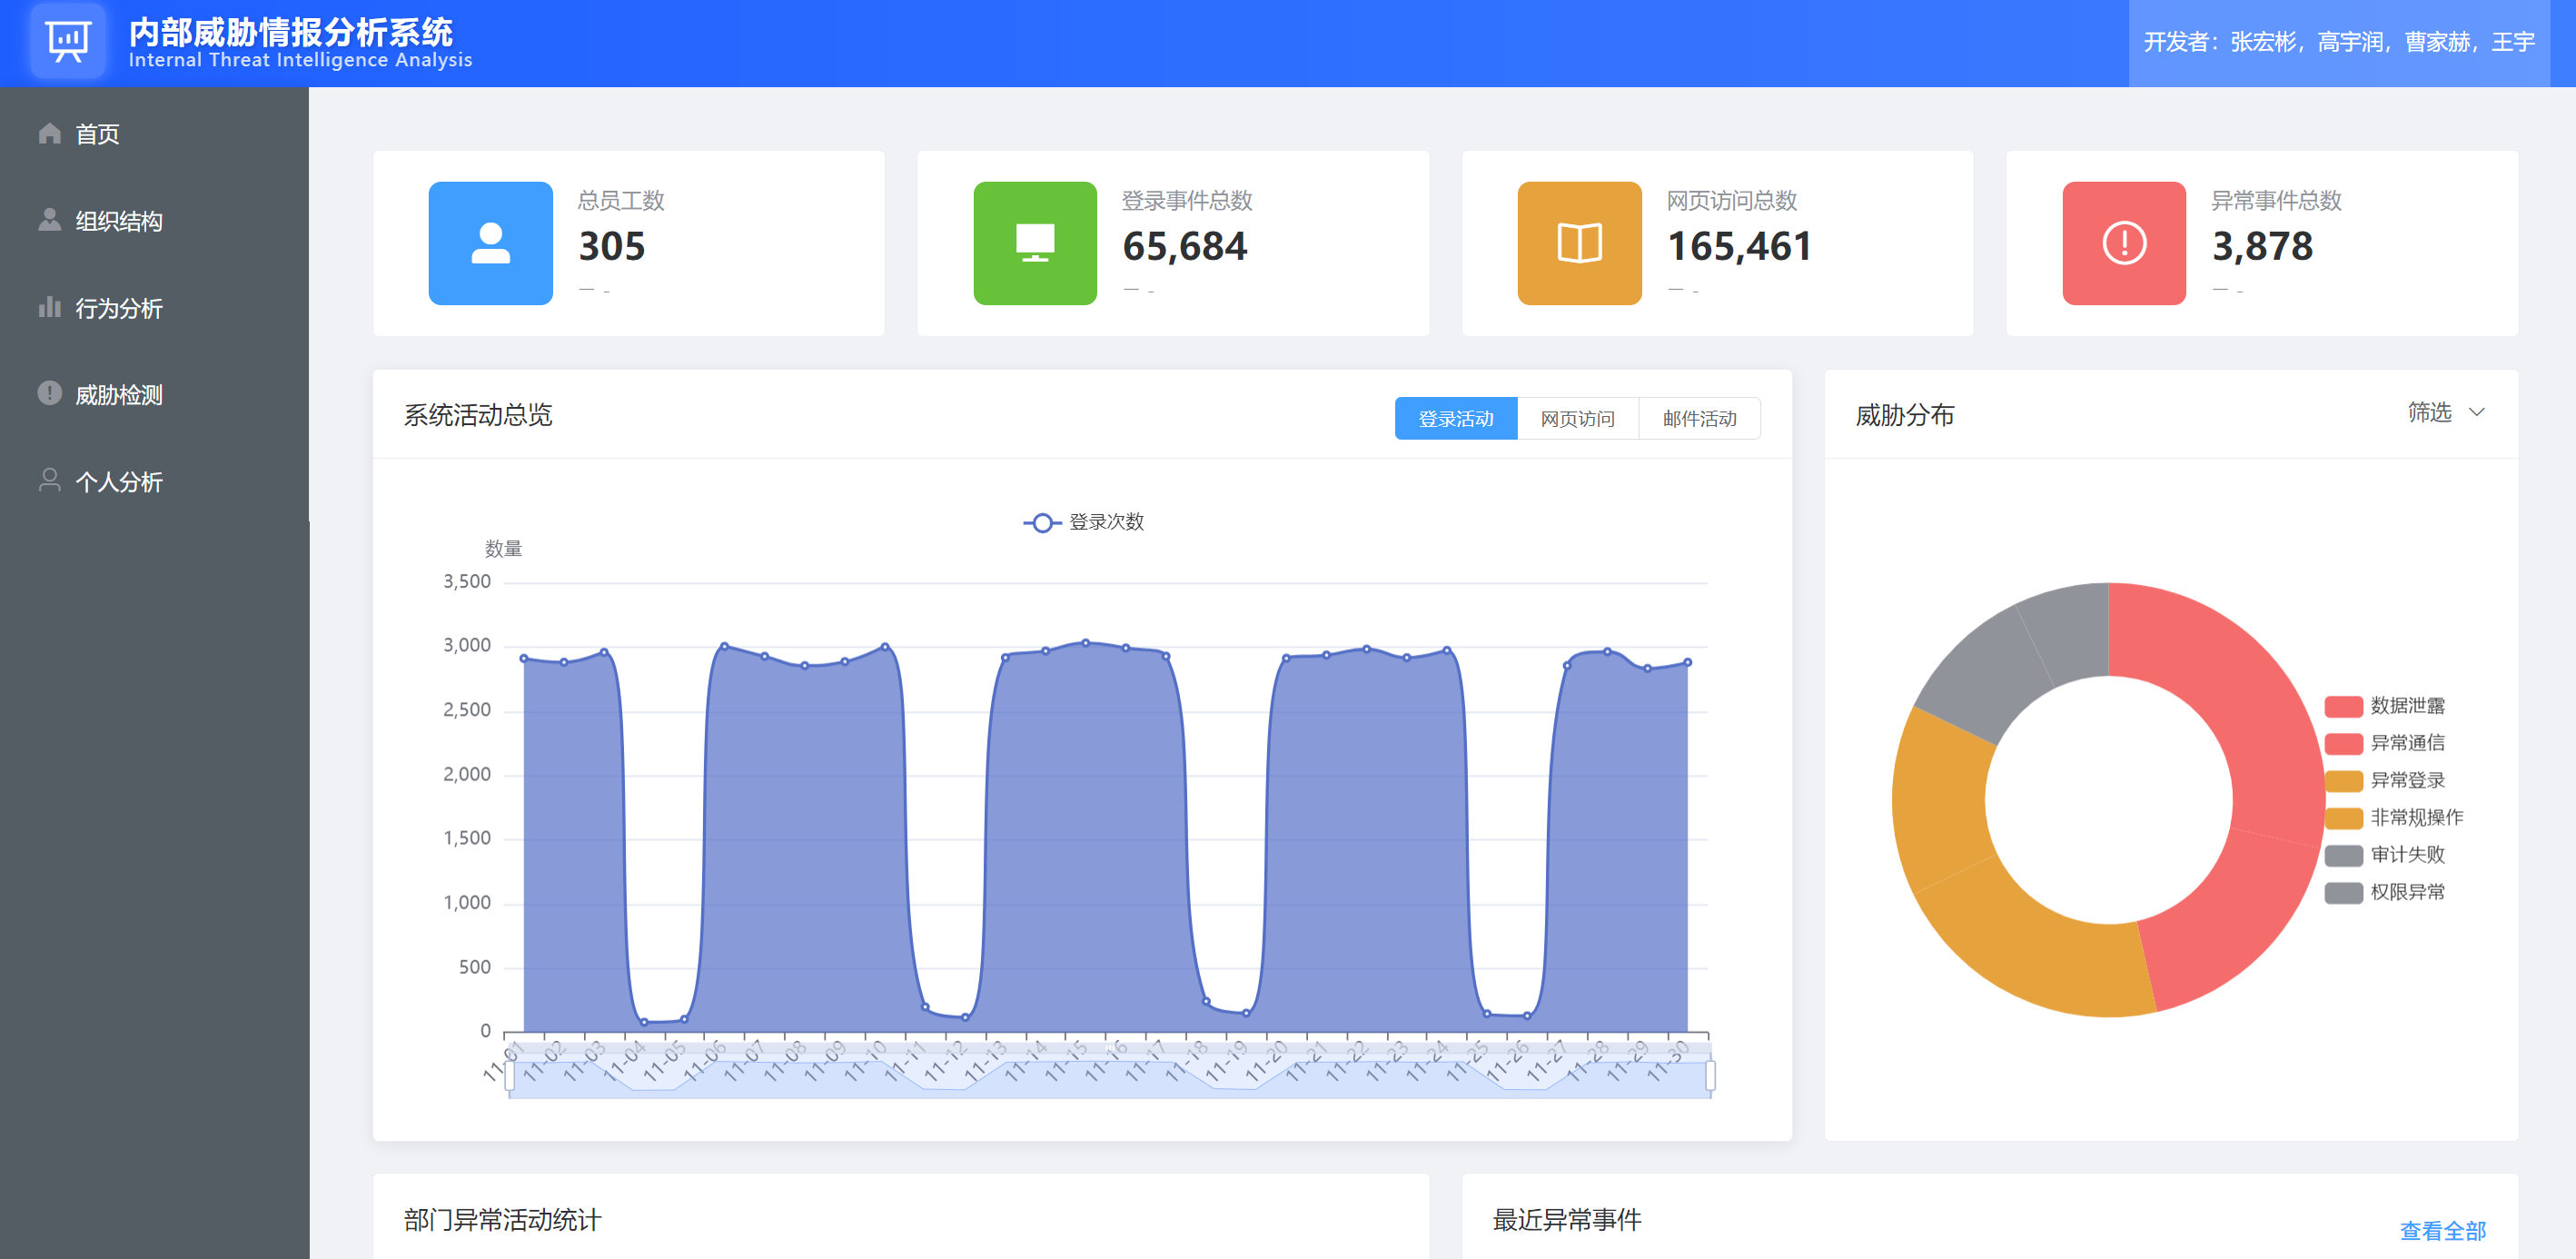
\includegraphics[width=\textwidth]{home.png}
        \caption{威胁情报总览}
        \label{fig:home_overview}
    \end{subfigure}
    \begin{subfigure}{0.48\textwidth}
        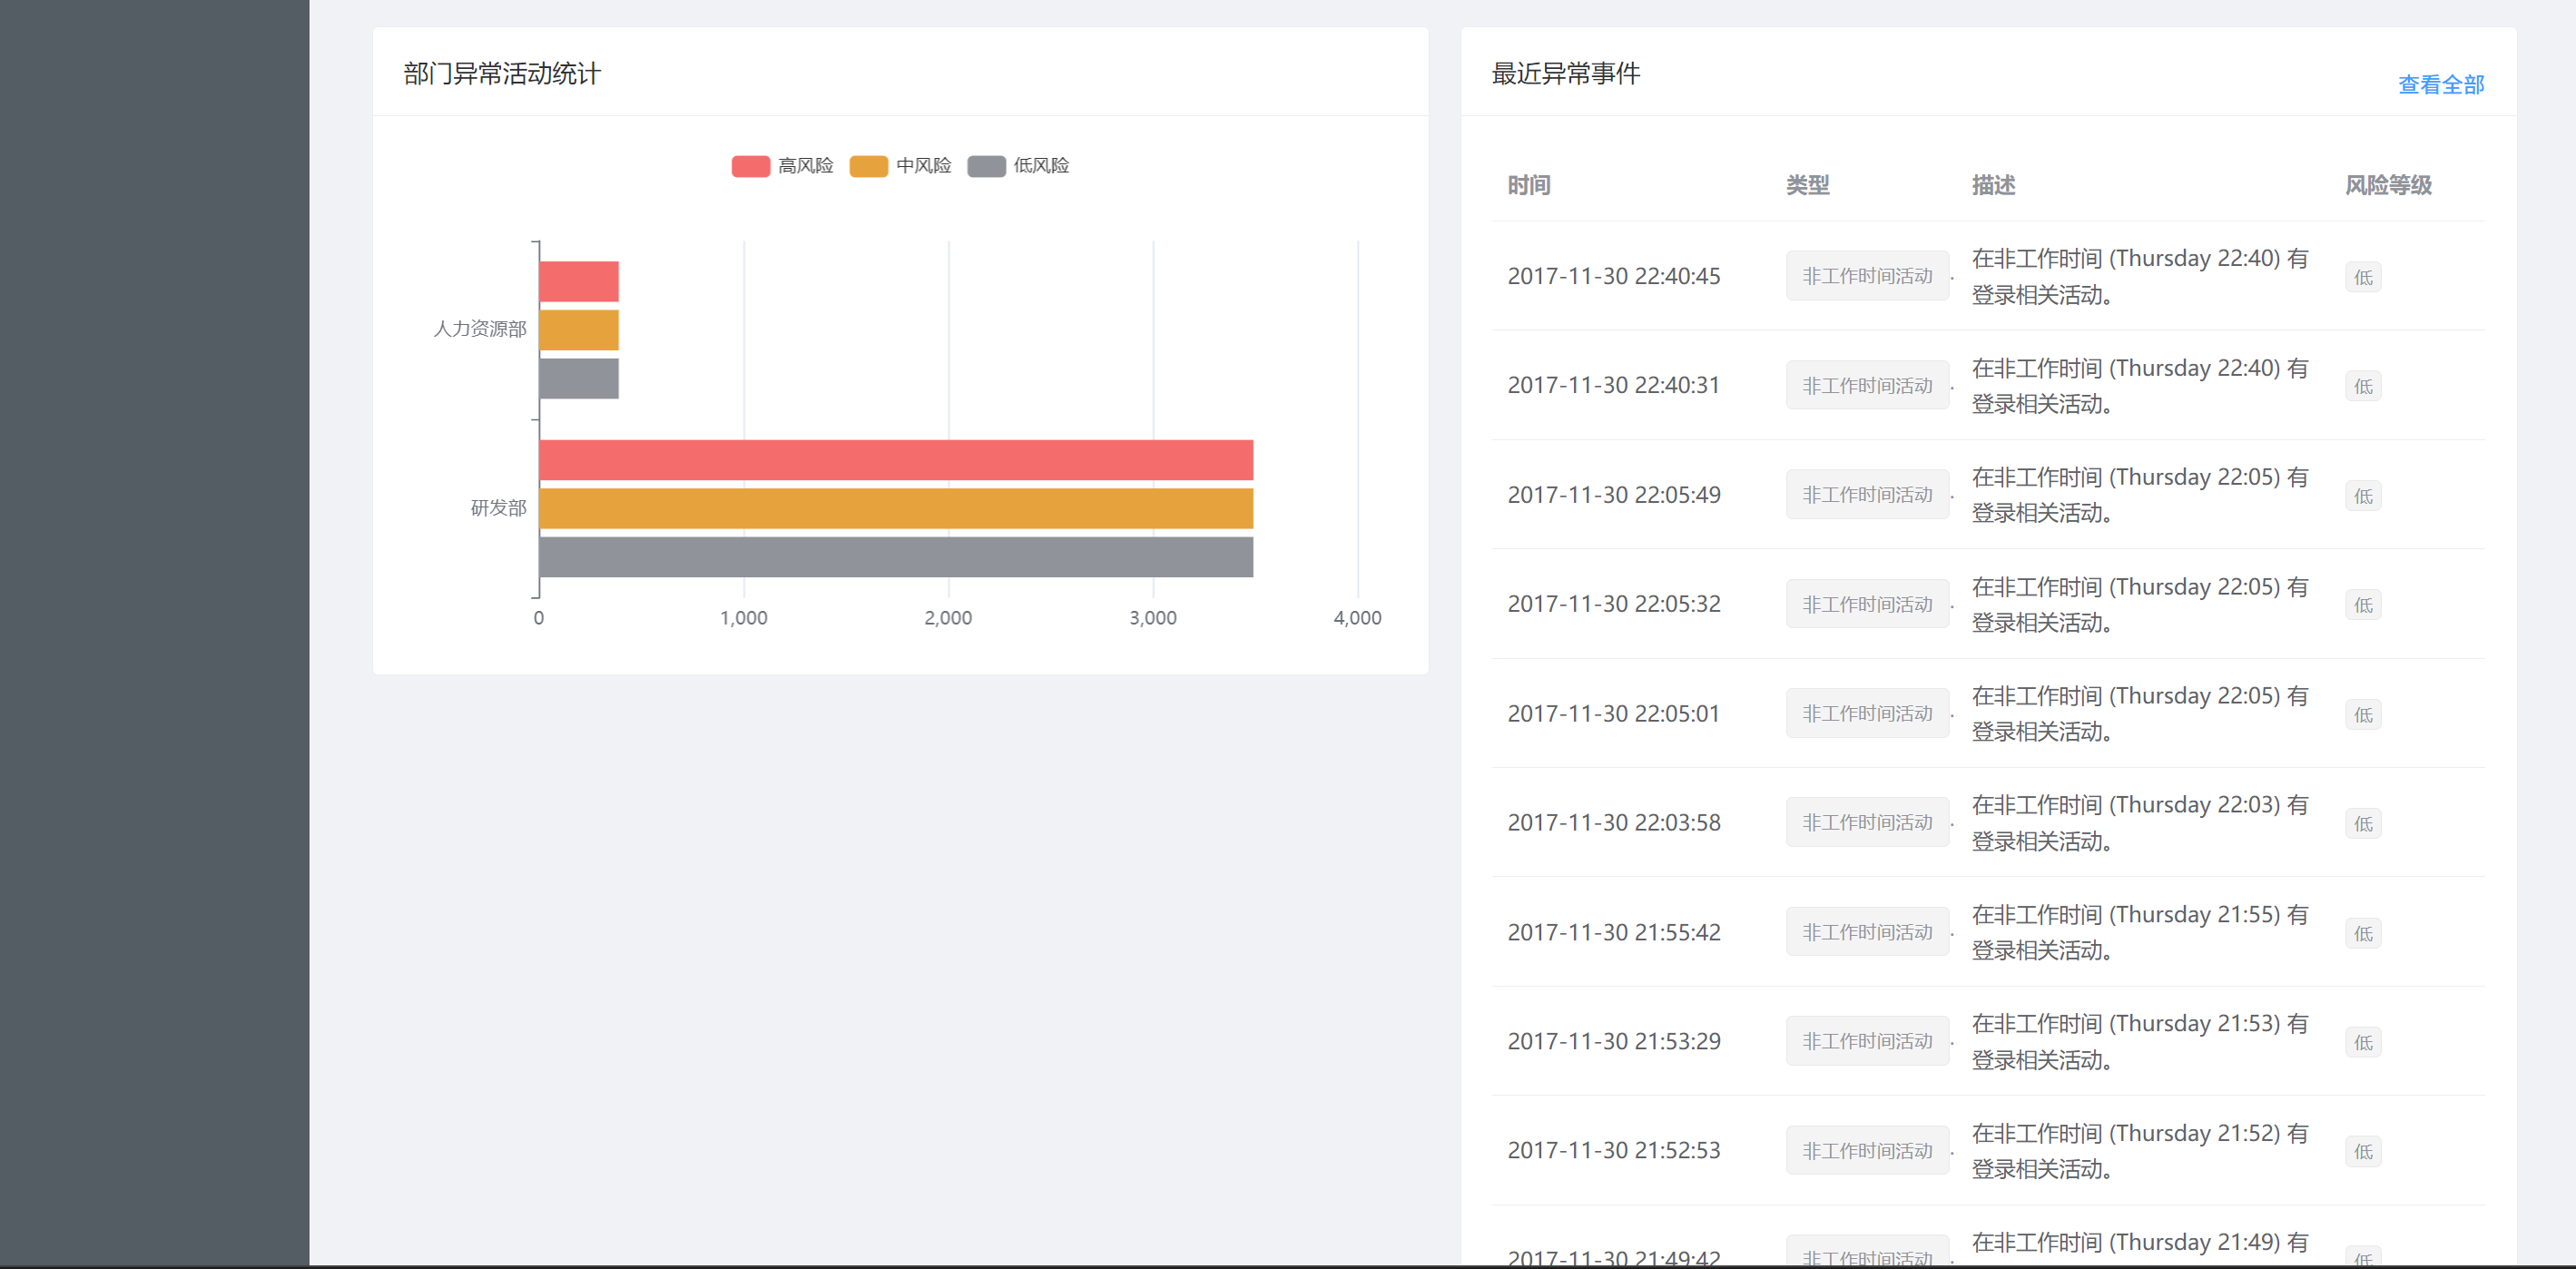
\includegraphics[width=\textwidth]{home_threat.png}
        \caption{威胁情报详情}
        \label{fig:home_threat}
    \end{subfigure}
    \caption{威胁情报分析仪表板}
    \label{fig:threat_dashboard}
\end{figure}

主要发现包括:
\begin{itemize}
    \item 研发部门是主要的攻击目标,特别是在产品发布前期
    \item 社会工程学攻击(如钓鱼邮件)是重要的入口点
    \item 内部威胁往往具有多维度的异常特征
    \item 及时的异常检测和响应对防止数据泄露至关重要
\end{itemize}

\section{结论与展望}
本报告通过构建完整的内部威胁情报分析框架,在理论创新和实践应用两个维度都取得了显著成果。在理论方法层面,我们提出的"数据-模型-认知"三层分析框架实现了从原始日志到可操作威胁情报的系统性转化。该框架不仅解决了多源异构数据的融合问题,还建立了从数据到知识的完整推导链条。特别地,我们开发的异常检测算法体系将统计建模和机器学习技术有机结合,显著提升了异常行为的识别准确率。在可视分析技术方面,我们设计的交互式分析方案突破了传统的静态展示模式,为分析人员提供了灵活的探索式分析工具,有效支持了复杂场景下的决策判断。

在实践应用层面,本报告达到的成果主要体现在三个方面。首先,在组织结构洞察方面,我们的分析框架不仅准确识别出了公司的三个核心部门及其职能特征,还通过社交网络分析方法揭示了部门间潜在的协作模式和信息流动规律。这些发现为优化组织结构和提升运营效率提供了数据支持。其次,在行为模式刻画方面,我们建立的时空基线模型实现了对员工活动模式的精确量化,这不仅有助于评估部门工作效率,还为异常行为检测提供了可靠的参考标准。最后,在威胁情报发现方面,我们成功识别出多类典型异常事件,并通过事件关联分析构建了完整的攻击链条,为企业安全防御提供了具有实践指导意义的建议。

展望未来,我们认为内部威胁情报分析还有三个重要的发展方向。在方法论层面,深度学习技术的引入将为异常检测带来新的突破。特别是在处理高维特征和复杂时序模式方面,深度学习模型展现出了显著优势。我们计划开发基于图神经网络的异常检测模型,以更好地捕捉员工行为网络中的异常模式。同时,智能化的关联分析算法将帮助分析人员更快速地识别潜在威胁。

在应用拓展方面,我们将重点关注数据源的扩展和实时分析能力的提升。通过整合更多类型的日志数据,如应用程序日志、系统日志等,可以构建更全面的威胁感知网络。同时,我们计划开发流式数据处理框架,支持大规模数据的实时分析,实现对威胁的及时发现和响应。此外,自动化的威胁响应机制也是未来重要的研究方向,我们将探索基于规则引擎和机器学习的智能响应策略。

在系统架构层面,我们将致力于提升分析平台的可扩展性和实用性。首先,通过优化数据处理和存储架构,提高系统处理大规模数据的能力。其次,增强系统的可扩展性,使其能够灵活适应不同规模企业的安全需求。最后,通过改进与现有安全设施的集成接口,实现威胁情报的无缝共享和联动响应。

基于本实践的发现,我们建议企业从技术、管理和流程三个维度强化内部安全防御体系。在技术层面,应重点加强对敏感数据的访问控制,实施更严格的网络准入策略,并部署先进的威胁检测系统。在管理层面,需要完善员工离职交接流程,加强安全意识培训,建立快速响应机制。在流程层面,应规范数据使用和传输流程,建立定期的安全审计制度,优化跨部门协作机制。

综上,通过本实践开发的可视分析系统,能够较好地完成本题的需求。

\end{document}